%!TEX TS-program = xelatex
\documentclass[notes,12pt, aspectratio=169]{beamer}

\usepackage{amsmath,amsfonts,amssymb,amsthm,mathtools}  % пакеты для математики
\usepackage{minted}

\usepackage[english, russian]{babel} % выбор языка для документа
\usepackage[utf8]{inputenc} % задание utf8 кодировки исходного tex файла
\usepackage[X2,T2A]{fontenc}        % кодировка

\usepackage{fontspec}         % пакет для подгрузки шрифтов
\setmainfont{Helvetica}  % задаёт основной шрифт документа

% why do we need \newfontfamily:
% http://tex.stackexchange.com/questions/91507/
\newfontfamily{\cyrillicfonttt}{Helvetica}
\newfontfamily{\cyrillicfont}{Helvetica}
\newfontfamily{\cyrillicfontsf}{Helvetica}

\usepackage{unicode-math}     % пакет для установки математического шрифта
% \setmathfont{Neo Euler} % шрифт для математики

\usepackage{polyglossia}      % Пакет, который позволяет подгружать русские буквы
\setdefaultlanguage{russian}  % Основной язык документа
\setotherlanguage{english}    % Второстепенный язык документа

% Шрифт для кода
\setmonofont[Scale=0.85]{Monaco}
\usepackage{verbments}

\usepackage{pgfpages}
% These slides also contain speaker notes. You can print just the slides,
% just the notes, or both, depending on the setting below. Comment out the want
% you want.
%\setbeameroption{hide notes} % Only slide
%\setbeameroption{show only notes} % Only notes
%\setbeameroption{show notes on second screen=right} % Both

\usepackage{array}

\usepackage{tikz}
\usepackage{verbatim}
\setbeamertemplate{note page}{\pagecolor{yellow!5}\insertnote}
\usetikzlibrary{positioning}
\usetikzlibrary{snakes}
\usetikzlibrary{calc}
\usetikzlibrary{arrows}
\usetikzlibrary{decorations.markings}
\usetikzlibrary{shapes.misc}
\usetikzlibrary{matrix,shapes,arrows,fit,tikzmark}

\usepackage{hyperref}
\usepackage{lipsum}
\usepackage{multimedia}
\usepackage{multirow}
\usepackage{dcolumn}
\usepackage{bbm}
\newcolumntype{d}[0]{D{.}{.}{5}}

\usepackage{changepage}
\usepackage{appendixnumberbeamer}
\newcommand{\beginbackup}{
   \newcounter{framenumbervorappendix}
   \setcounter{framenumbervorappendix}{\value{framenumber}}
   \setbeamertemplate{footline}
   {
     \leavevmode%
     \hline
     box{%
       \begin{beamercolorbox}[wd=\paperwidth,ht=2.25ex,dp=1ex,right]{footlinecolor}%
%         \insertframenumber  \hspace*{2ex} 
       \end{beamercolorbox}}%
     \vskip0pt%
   }
 }
\newcommand{\backupend}{
   \addtocounter{framenumbervorappendix}{-\value{framenumber}}
   \addtocounter{framenumber}{\value{framenumbervorappendix}} 
}

% для имитации питоновского синтаксиса 
\newcommand{\pgr}[1]{{\color{green} \textbf{#1}}}


%%%%%%%%%% Работа с картинками %%%%%%%%%
\usepackage{graphicx}                  % Для вставки рисунков
\usepackage{graphics}
\graphicspath{{images/}}    % можно указать папки с картинками
\usepackage{wrapfig}                   % Обтекание рисунков и таблиц текстом

\usepackage[space]{grffile}
\usepackage{booktabs}

% These are my colors -- there are many like them, but these ones are mine.
\definecolor{blue}{RGB}{0,114,178}
\definecolor{red}{RGB}{213,94,0}
\definecolor{yellow}{RGB}{240,228,66}
\definecolor{green}{RGB}{0,128, 0}

\hypersetup{
  colorlinks=true,
  linkbordercolor = {white},
  urlcolor=blue
}


%% I use a beige off white for my background
\definecolor{MyBackground}{RGB}{255,253,218}

%% Uncomment this if you want to change the background color to something else
%\setbeamercolor{background canvas}{bg=MyBackground}

%% Change the bg color to adjust your transition slide background color!
\newenvironment{transitionframe}{
  \setbeamercolor{background canvas}{bg=yellow}
  \begin{frame}}{
    \end{frame}
}

\setbeamercolor{frametitle}{fg=blue}
\setbeamercolor{title}{fg=black}
\setbeamertemplate{footline}[frame number]
\setbeamertemplate{navigation symbols}{} 
\setbeamertemplate{itemize items}{-}
\setbeamercolor{itemize item}{fg=blue}
\setbeamercolor{itemize subitem}{fg=blue}
\setbeamercolor{enumerate item}{fg=blue}
\setbeamercolor{enumerate subitem}{fg=blue}
\setbeamercolor{button}{bg=MyBackground,fg=blue,}


% If you like road maps, rather than having clutter at the top, have a roadmap show up at the end of each section 
% (and after your introduction)
% Uncomment this is if you want the roadmap!
% \AtBeginSection[]
% {
%    \begin{frame}
%        \frametitle{Roadmap of Talk}
%        \tableofcontents[currentsection]
%    \end{frame}
% }
\setbeamercolor{section in toc}{fg=blue}
\setbeamercolor{subsection in toc}{fg=red}
\setbeamersize{text margin left=1em,text margin right=1em} 

% списки, которые растягиваются на всю величину слайда 
\newenvironment{wideitemize}{\itemize\addtolength{\itemsep}{10pt}}{\enditemize}

\usepackage{xcolor}

% Syntax: \colorboxed[<color model>]{<color specification>}{<math formula>}
\newcommand*{\colorboxed}{}
\def\colorboxed#1#{%
	\colorboxedAux{#1}%
}

\newcommand*{\colorboxedAux}[3]{%
	% #1: optional argument for color model
	% #2: color specification
	% #3: formula
	\begingroup
	\colorlet{cb@saved}{.}%
	\color#1{#2}%
	\boxed{%
		\color{cb@saved}%
		#3%
	}%
	\endgroup
}

\usepackage{pgfplots}
\usepackage{tikz}

\DeclareMathOperator{\logloss}{logloss}
\DeclareMathOperator{\Softmax}{Softmax}

\title[]{\textcolor{blue}{Глубокое обучение и вообще}}
\author{Ульянкин Филипп}
\date{\today}

\usepackage{ulem}
\usepackage{MnSymbol,wasysym}

\begin{document}

%%% TIKZ STUFF
\tikzset{   
        every picture/.style={remember picture,baseline},
        every node/.style={anchor=base,align=center,outer sep=1.5pt},
        every path/.style={thick},
        }
\newcommand\marktopleft[1]{%
    \tikz[overlay,remember picture] 
        \node (marker-#1-a) at (-.3em,.3em) {};%
}
\newcommand\markbottomright[2]{%
    \tikz[overlay,remember picture] 
        \node (marker-#1-b) at (0em,0em) {};%
}
\tikzstyle{every picture}+=[remember picture] 
\tikzstyle{mybox} =[draw=black, very thick, rectangle, inner sep=10pt, inner ysep=20pt]
\tikzstyle{fancytitle} =[draw=black,fill=red, text=white]
%%%% END TIKZ STUFF

% Title Slide

\begingroup
\setbeamercolor{background canvas}{bg = black}
\begin{frame}[plain]
\begin{center}
	\Huge{\color{red}{ВНИМАНИЕ!}}
\end{center}

\begin{center}
	\color{white}{ДАННЫЙ КУРС СОДЕРЖИТ БОЛЬШОЕ КОЛИЧЕСТВО РАЗНООБРАЗНОГО КОДА И ЗАДАНИЙ ДЛЯ САМОСТОЯТЕЛЬНОГО РЕШЕНИЯ. \\
		\vspace{3mm}
		НА ПЕРВЫЙ ВЗГЛЯД ОН МОЖЕТ ПОКАЗАТЬСЯ СЛОЖНЫМ И ТРАВМИРОВАТЬ НЕПОДГОТОВЛЕННУЮ ПСИХИКУ. ТАКЖЕ ОН СОДЕРЖИТ БОЛЬШОЕ КОЛИЧЕСТВО НЕУДАЧНЫХ ШУТОК И НЕУМЕСТНЫХ ОТСЫЛОК. \\ 
		\vspace{3mm}
		В СВЯЗИ С ЭТИМ КУРС НЕ РЕКОМЕНДУЕТСЯ ПРОСЛУШИВАТЬ \ldots{ } НИКОМУ.}
\end{center}
\end{frame}
\endgroup


\begin{frame}
\maketitle
\centering \textbf{\color{blue} Посиделка 1:}  вводная
\end{frame}

{
	\usebackgroundtemplate{ 
		\hspace{3cm}	
\includegraphics[height=\paperheight]{ya.jpg}}
	\begin{frame}
\end{frame}
}

\begin{frame}{Agenda}
\begin{wideitemize}
	\item О том каким будет курс + что почитать/посмотреть
	\item  Фреймворки для нейроночек
	\item  Немного истории и важные тренды 
	\item От регрессии к нейросетке
	\item Нейросетки - конструктор Lego
	\item Учим свою первую нейросетку 
\end{wideitemize} 
\end{frame}


\begin{transitionframe}
	\begin{center}
	\centering 
\includegraphics[scale = 0.03]{pac-man.png}	\Huge Правила игры и почиташки
	\end{center}
\end{transitionframe}


 \begin{frame}{Про пары}
\begin{wideitemize}
	\item  что-то неясно $\Rightarrow$ \alert{ ПЕРЕБЕЙ И СПРОСИ}
	
	\item  на парах смотрим презы, пишем код, решаем задачи
	
	\item  будет много математики  \blacksmiley{}
	
	\item  на кодинговые пары лучше приходить со своим ноутбуком
	
	\item все материалы можно найти на  \href{https://github.com/FUlyankin/neural_nets_econ}{страничке курса}
\end{wideitemize} 
\end{frame}

%\begin{frame}{Про домашки}
%\begin{wideitemize}
%	\item  Не делаешь сам $\Rightarrow$ никогда не научишься $\Rightarrow$ \sout{большие} огромные домашки
%	
%	\item  Домашки делаются в командах по два человека, их около 8 штук, баллы ставятся на команду. Можно набрать $> 200$ баллов. Если вы набрали $100$, у вас десятка. 
%	
%	\item  $N \le 6$ человек из топа списка свожу почилить на крышу Яндекса. 
%\end{wideitemize} 
%\end{frame}

\begin{frame}{Что почитать про нейронки в первую очередь}
\begin{columns}
	\begin{column}{0.5\textwidth}
\begin{center}
	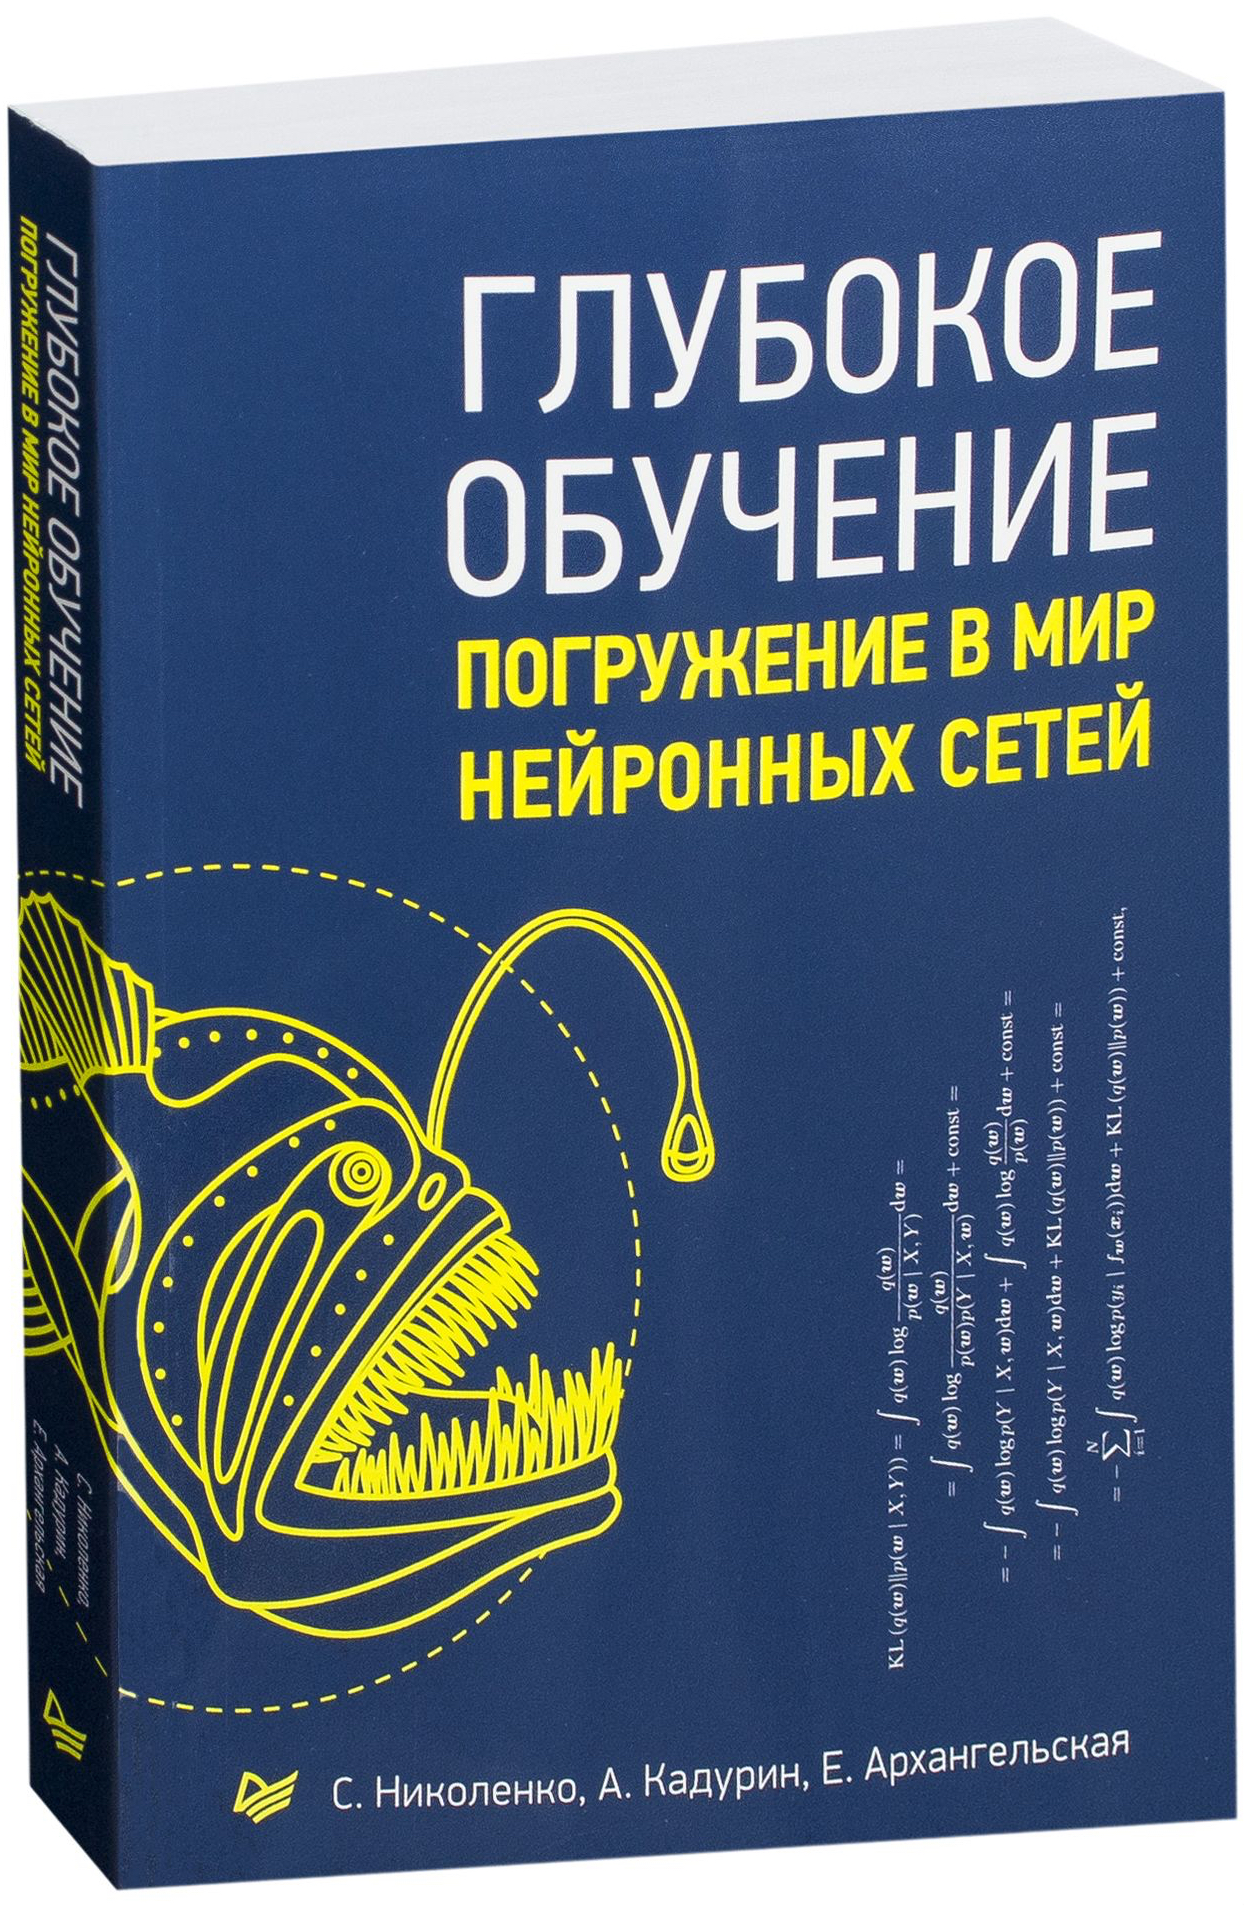
\includegraphics[width=0.5\textwidth]{book1.jpg}  
	
	\footnotesize Баланс математики и практики, \\ код устарел (tensorflow 1.14)
\end{center}

	\end{column}
	\begin{column}{0.5\textwidth}
		\begin{center}
			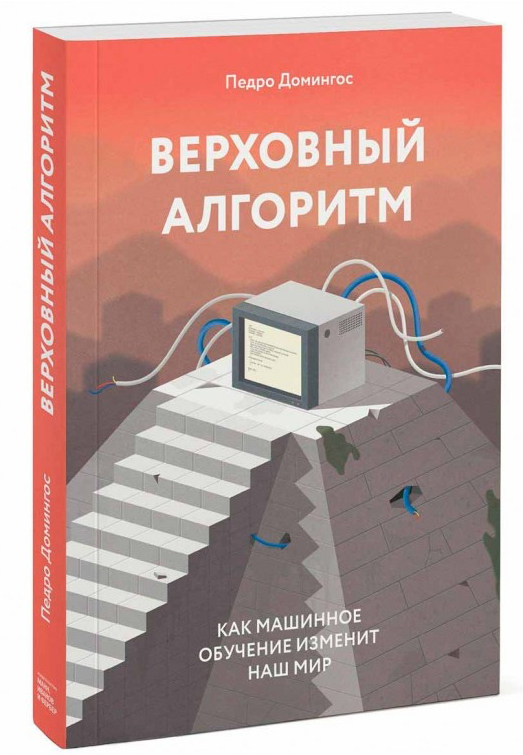
\includegraphics[width=0.5\textwidth]{book2.jpg} 
			
			\footnotesize Философия и история ML
		\end{center}
	\end{column}
\end{columns}
\end{frame} 


\begin{frame}{Что почитать про нейронки в первую очередь}
\begin{columns}
	\begin{column}{0.5\textwidth}
		\begin{center}
			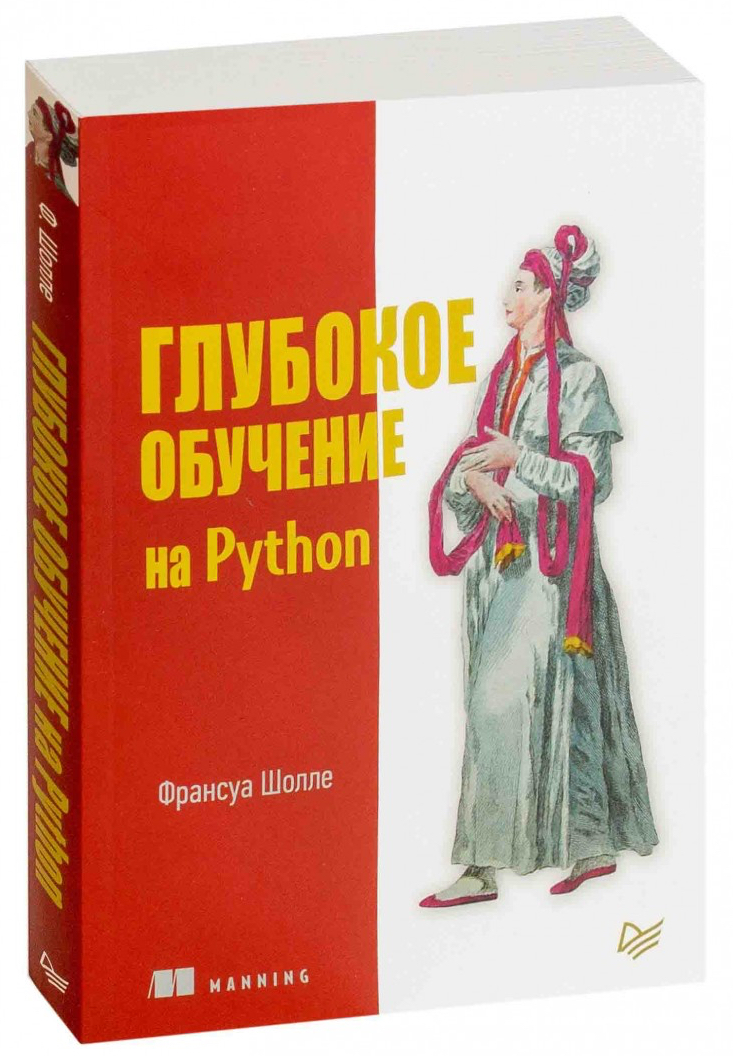
\includegraphics[width=0.5\textwidth]{book3.jpg}
			
	\footnotesize Простая практика на Keras
		\end{center}
	\end{column}
	\begin{column}{0.5\textwidth}
		\begin{center}
			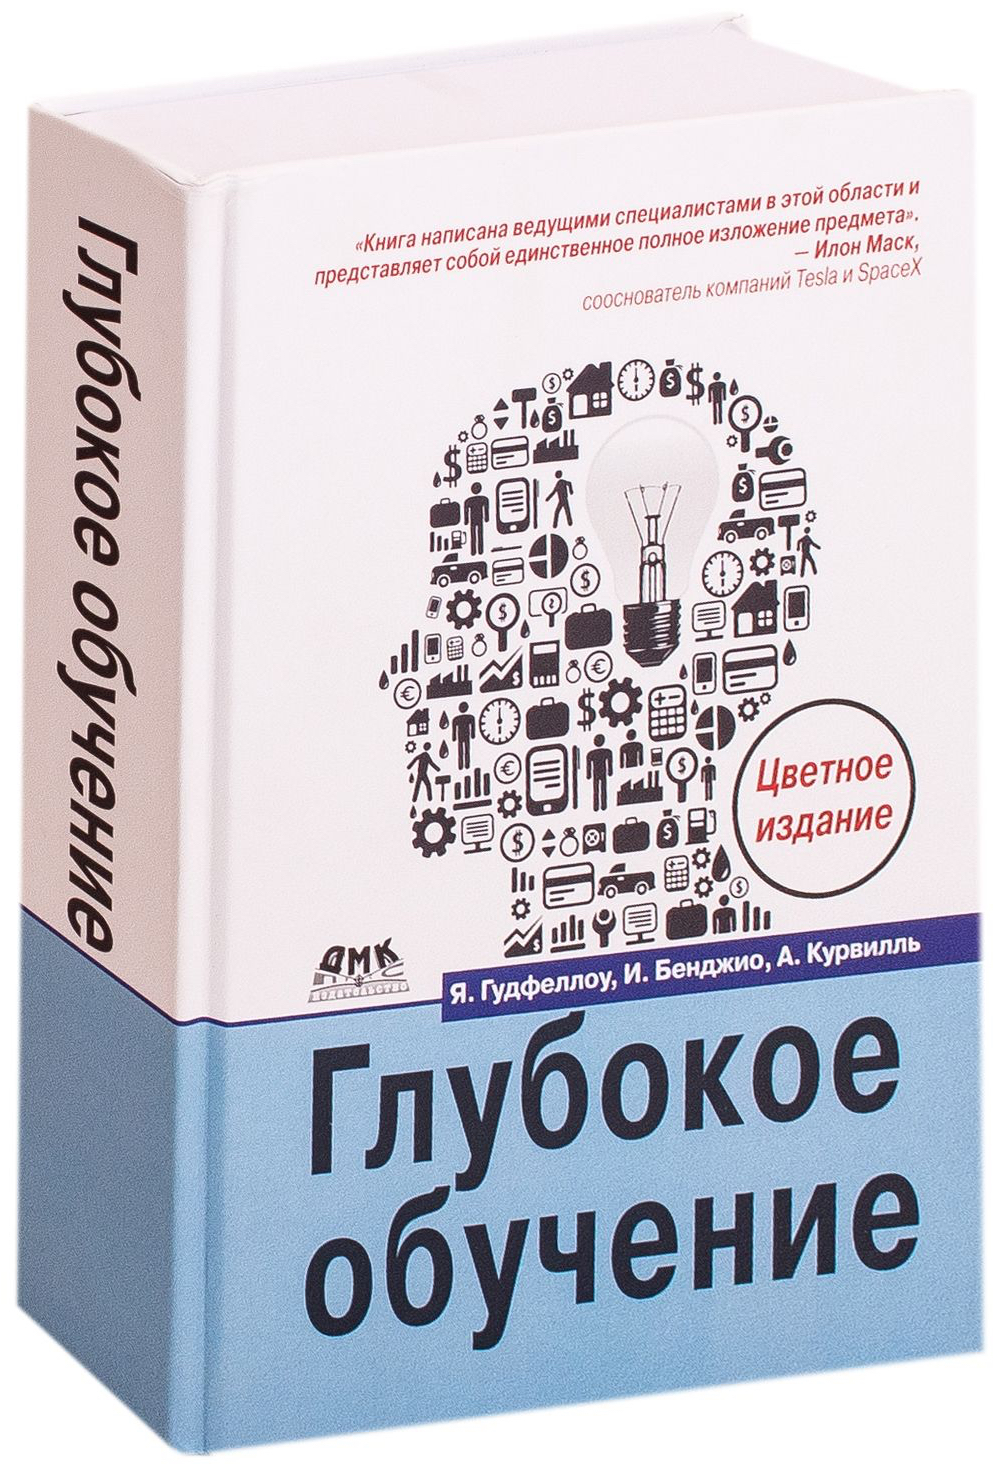
\includegraphics[width=0.5\textwidth]{book4.jpg}
			
	\footnotesize Хардкорная математика, \\ библия глубокого обучения
		\end{center}
	\end{column}
\end{columns}
\end{frame} 


\begin{frame}{Что посмотреть  про нейронки}
\begin{wideitemize} 
\item Если ничего не знаете про машинное обучение, смотрите \href{https://www.coursera.org/specializations/machine-learning-data-analysis}{вводный курс от Яндекса и МФТИ.} \alert{Для тех, кто мало знает про ML.}

\item  \href{https://www.coursera.org/specializations/aml}{Advanced ML от Яндекса.} Там есть очень разные специфические курсы. Первый из них про нейронки. Код на Tensorflow. Версия библиотеки там пока что старая.  \alert{Для тех, кто хочет развиваться дальше.}

\item  \href{https://www.coursera.org/specializations/deep-learning} {Нейронные сети от Andrew Ng.} Когда ML ещё не был таким модным, все смотрели его лекции. \alert{Для тех, кто хочет всё делать медленно и непринуждённо.}

\item  \href{https://github.com/yandexdataschool/Practical_DL/tree/master}{Курс нейронок, который читают в ШАД и Сколтехе.} Есть варианты кода на разных фреймворках. Есть видео лекций на русском и английском. \alert{Для тех, кто хочет посмотреть как читают курс по DL  в ШАД.}
\end{wideitemize} 
\end{frame} 


\begin{frame}{Что посмотреть  про нейронки}
\begin{wideitemize} 
	
	\item Бесплатный \href{https://www.udacity.com/course/intro-to-tensorflow-for-deep-learning--ud187}{курс по tf от Google.} Короткий. Покрывает весь базовый Keras. Все тетрадки выложены в colab. Есть странные интервью.  \alert{Для тех, кто  хочет быстро зашарить keras.}
	
	\item Бесплатный \href{https://stepik.org/course/50352/syllabus}{курс по pytorch от Samsung.}  Вводный курс в нейросетки на pytorch. \alert{Для тех, кто  хочет писать на pytorch.}
	
	\item  \href{https://dlcourse.ai}{Deep learning на пальцах.} Лекции из кремниевой долины. Задания на pytorch для самостоятельного решения.   \alert{Для тех, кто  хочет посмотреть няшные простые стримчики про нейронки.}
	
	\item \href{http://rusneuro.net/novosti/v-mfti-prohodit-kurs-theoretical-deep-learning-ot-ipavlov}{Курс от IPavlov} Есть вводный курс, есть хардкорный курс.  Лично я заленился и не проходил, хотя регистрировался. 
\end{wideitemize} 
\end{frame} 


\begin{frame}{Структура курса}
\begin{center}
\begin{tikzpicture}[every node/.style={inner sep=0,outer sep=0}]
\node (B) at (0,0) {
\includegraphics[scale=.2]{frank.png}};

\node[circle, fill=red!50!black, opacity=.5, minimum size=.4cm] (nuc) at (B) {};
\node[circle, fill=red!50!black, opacity=.5, minimum size=.4cm] (cyt) at ($(B)+(.4,.4)$) {};
\node[circle, fill=green!25!black, opacity=.5, minimum size=.4cm] (cha) at ($(B)+(.8,-.6)$) {};
\node[circle, fill=green!25!black, opacity=.5, minimum size=.4cm] (mem) at ($(B)+(.4,-1)$) {};

\node[right=1cm of B.north east, align=left, text width=6cm, font=\scriptsize, fill=yellow] (C1) {
	\setbeamertemplate{itemize items}[circle]
	\setbeamercolor{local structure}{fg=red!50!black}\color{red!50!black}
	\setlength{\leftmargini}{6pt}
	\setlength{\labelsep}{1pt}
	\begin{itemize}
	\color{red!50!black}
	\itemsep1pt
	\item \alert{Базовая часть курса:}
	\item От регрессии к нейросети, Keras
	\item 50 оттенков градиентного спуска, Backpropagation
	\item Введение в Tensorflow
	\item Эвристики и приёмы для обучения сеток
	\end{itemize}
};
\draw[thick,decorate,decoration={brace,mirror,amplitude=5pt}, color=red!50!black] (C1.north west) -- (C1.south west) node[midway] {};

\node[right=0.5cm of B.east, align=left, shift={(0cm,-1.5cm)}, text width=6cm, font=\scriptsize, fill=yellow] (C2) {
	\setbeamertemplate{itemize items}[circle]
	\setbeamercolor{local structure}{fg=green!25!black}\color{red!50!black}
	\setlength{\leftmargini}{6pt}
	\setlength{\labelsep}{1pt}
	\begin{itemize}
	\color{green!25!black}
	\itemsep1pt
	\item \alert{Разные архитектуры:}
	\item  Свёрточные сети, локализация, сегментация, перенос стиля
	\item  Автокодировщики, генеративные модели
	\item  Рекурентные нейронные сетки
	\item  Введение в NLP, эмбединги, автопереводы, трансформеры
	\item  Обучение с подкреплением (немношка)
	\end{itemize}
};
\draw[thick,decorate,decoration={brace,mirror,amplitude=5pt}, color=green!25!black] (C2.north west) -- (C2.south west) node[midway] {};

\path[->, >=latex, red!50!black, opacity=.6, line width=1pt] {[out=350,in=180]
	(nuc) edge ($(C1.west)-(.2,0)$)
	(cyt) edge ($(C1.west)-(.2,0)$)};
\path[->, >=latex, green!25!black, opacity=.6, line width=1pt] {[out=350,in=180]
	(cha) edge ($(C2.west)-(.2,0)$)
	(mem) edge ($(C2.west)-(.2,0)$)};
\end{tikzpicture}
\end{center}
\end{frame}


\begin{transitionframe}
	\begin{center}
		\Huge Фреймворки для Deep Learning
	\end{center}  
	\centering \href{https://vk.com/skialz}{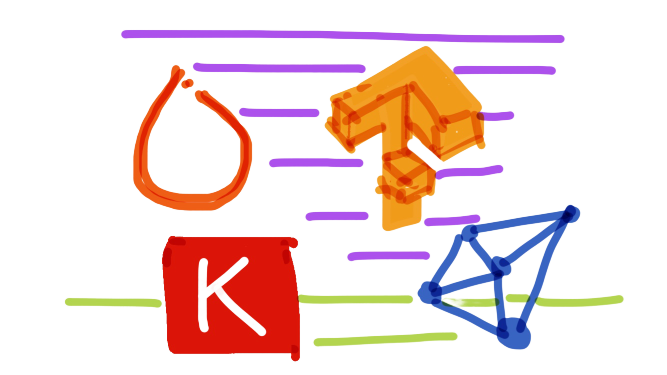
\includegraphics[scale = 0.15]{frameworks_pr.png}}
\end{transitionframe}

% переделать в виде таблицы, а то кривовато  (А, ПОХУЙ!)
\begin{frame}{Фрэймворки}
\begin{columns}[T] % align columns
	\begin{column}{.33\textwidth}
		\centering 	
\includegraphics[width=.6\linewidth]{theano.png} \\
		\mbox{ } \\
		\centering 	
\includegraphics[width=.6\linewidth]{Logo_Mila.png} \\
		\mbox{ } \\
		Монреальский университет (2007) \\ 
		\mbox{ } \\
		Static Computational Graph 
	\end{column}%
	\hfill%
	\begin{column}{.33\textwidth}
		\centering 	
\includegraphics[width=.7\linewidth]{tensorflow.png} \\
		\mbox{ } \\
		\centering 	
\includegraphics[width=.6\linewidth]{google.png} \\
		\mbox{ } \\	
		Google (2011, открыта с 2015, с 2019 tf 2.0) \\ 
		\mbox{ } \\
		\sout{Static}  Dynamic Computational Graph 
	\end{column}%
	\hfill%
	\begin{column}{.33\textwidth}
		\centering 	
\includegraphics[width=.7\linewidth]{pytorch.png} \\
		\mbox{ } \\
		\centering 	
\includegraphics[width=.3\linewidth]{facebook.png} \\
		\mbox{ } \\
		Facebook (2016) \\ 
		\mbox{ } \\
		Dynamic Computational Graph 
	\end{column}%
\end{columns}
\end{frame}


\begin{frame}{Обёртки}
\begin{center}
\begin{columns}[T] % align columns
	\begin{column}{.48\textwidth}
		\centering 	
		Сначала обёртка для Theano, потом для Tensorflow, сейчас фактически часть Tensorflow \\ 
		\mbox{  } \\
		
\includegraphics[width=.5\linewidth]{keras.png} \\
	\end{column}%
	\hfill%
	\begin{column}{.48\textwidth}
		\centering 	
		Обёртка для Theano \\ 
		\mbox{  } \\
		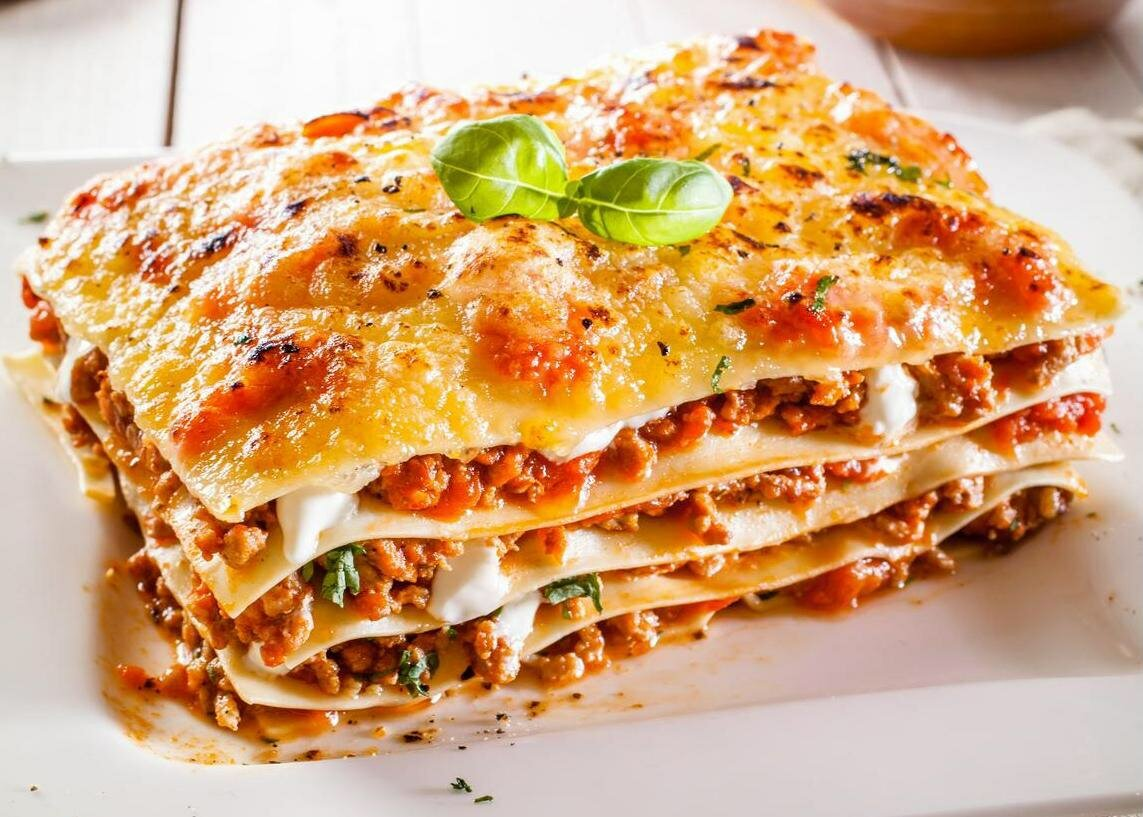
\includegraphics[width=.5\linewidth]{lasagne.jpeg} \\
	\end{column}%
\end{columns}
\end{center}

\vspace{2.5cm}
% \vfill % чёт не работает 

\scriptsize
Лекция про фрэймворки на русском (из  далёкого 2017 года): \color{blue} \url{https://www.youtube.com/watch?v=ghZyptkanB0} 
\end{frame}


% Переделать слайд нормально, блин 
\begin{frame}{Подходы к вычислениям}
\begin{center}
	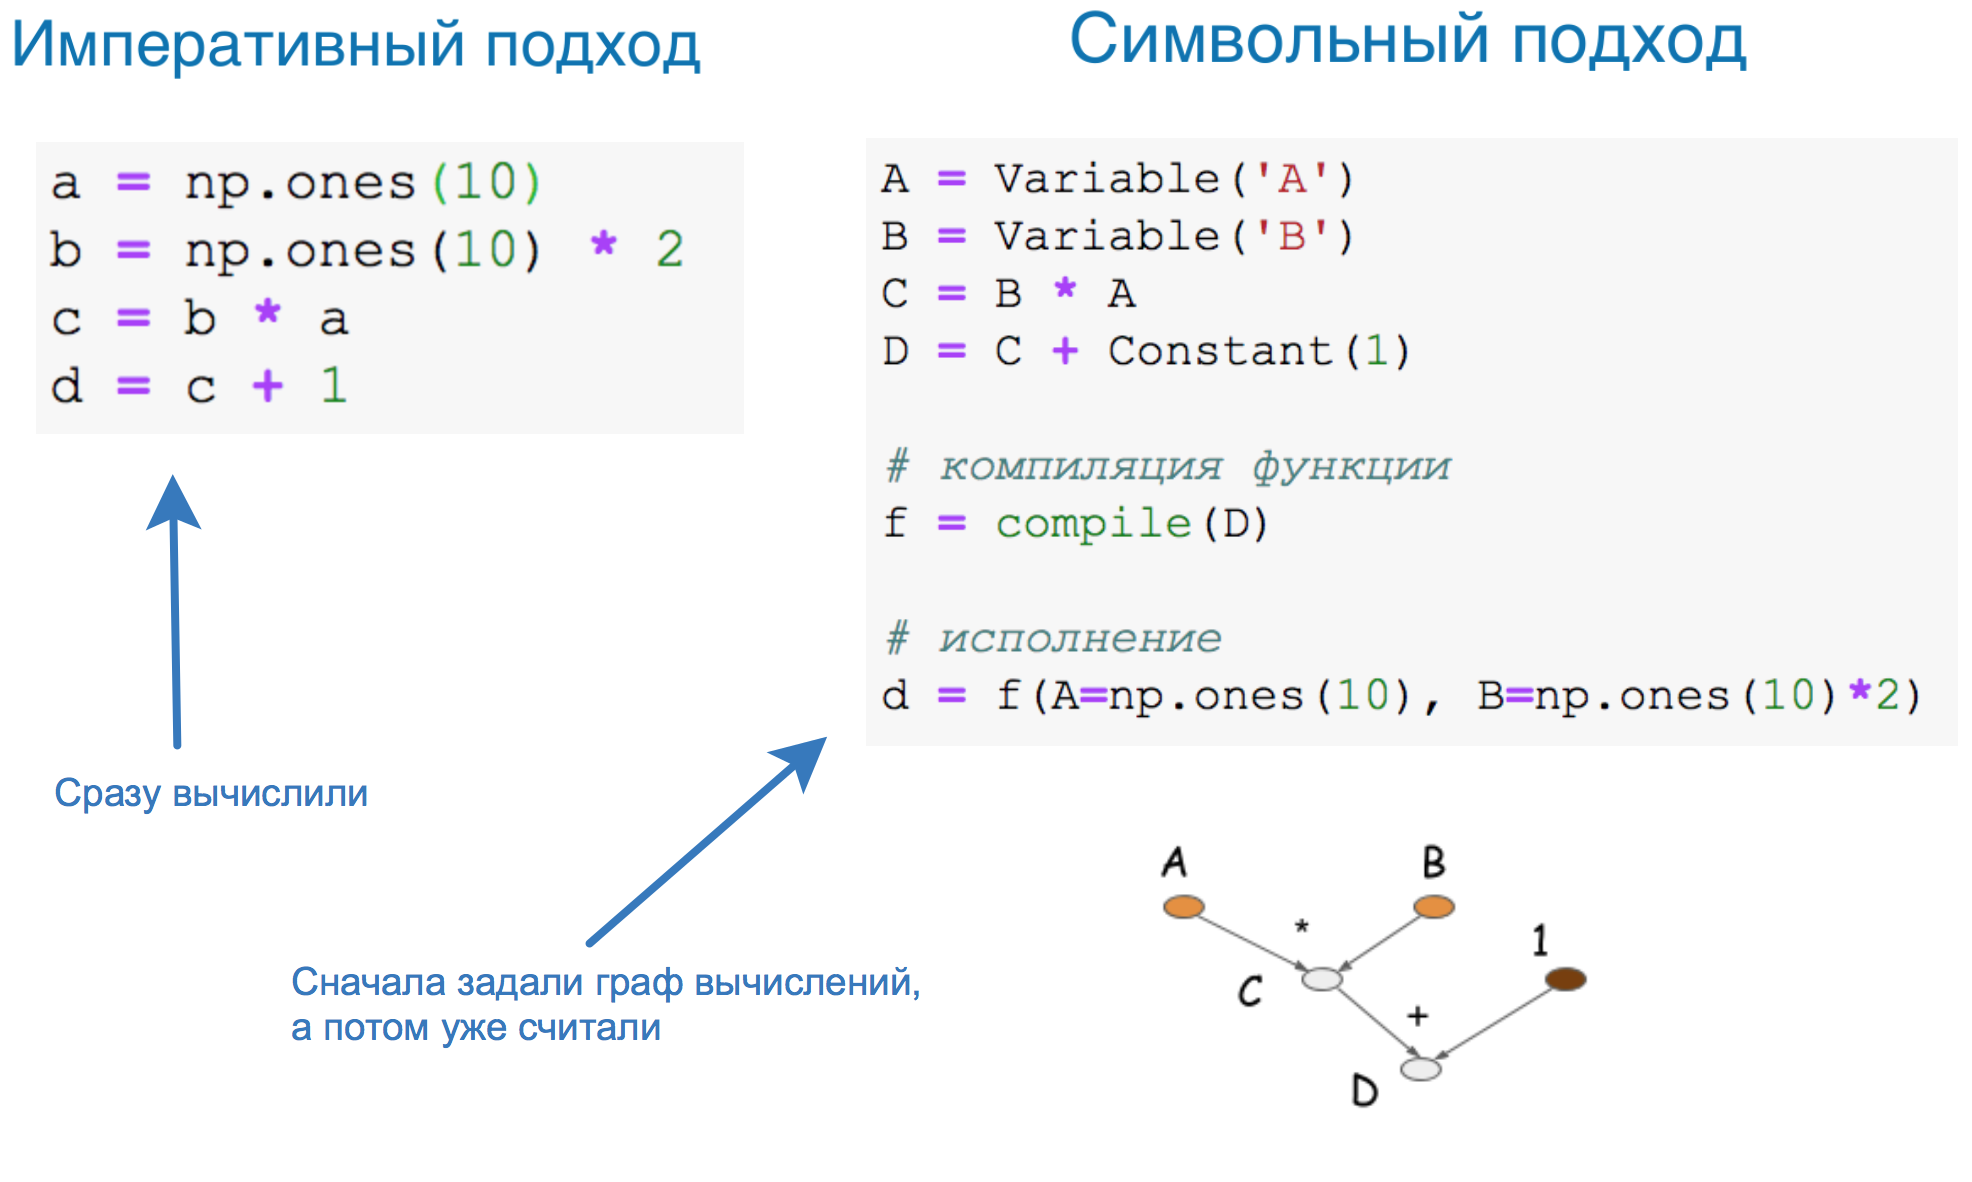
\includegraphics[width=.9\linewidth]{graph.png}
\end{center}
\end{frame} 


\begin{frame}{Символьный подход}
\begin{wideitemize}
\item[+] Легко строить сеть из вычислений и автоматически искать по ней производные \alert{(быстрая и простая оптимизация)}

\item[+] Более эффективные вычисления, как по памяти, так и по скорости (на этапе компиляции можно выявить неиспользуемые переменные, найти места для переиспользования и тп) 

\item Довольно сложно искать ошибки из-за того, что cначала задаётся граф вычислений
\end{wideitemize}
\end{frame} 


\begin{frame}{Мощь библиотек }

\begin{columns}[T] % align columns
	\begin{column}{.48\textwidth}
		\centering  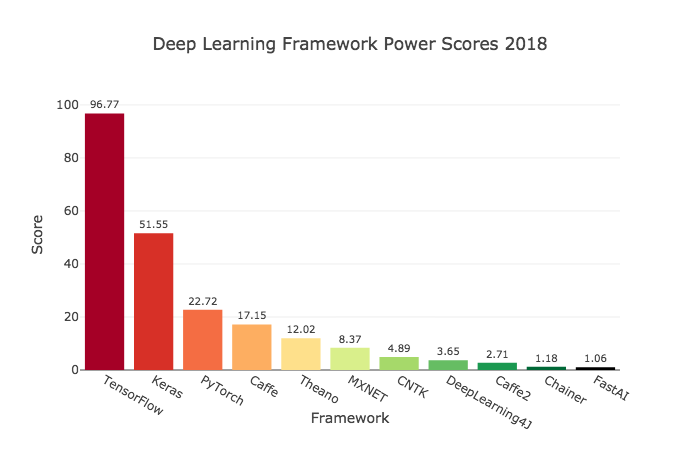
\includegraphics[width=.9\linewidth]{frameworks.png}
	\end{column}%
	\hfill%
	\begin{column}{.48\textwidth}
		\centering 	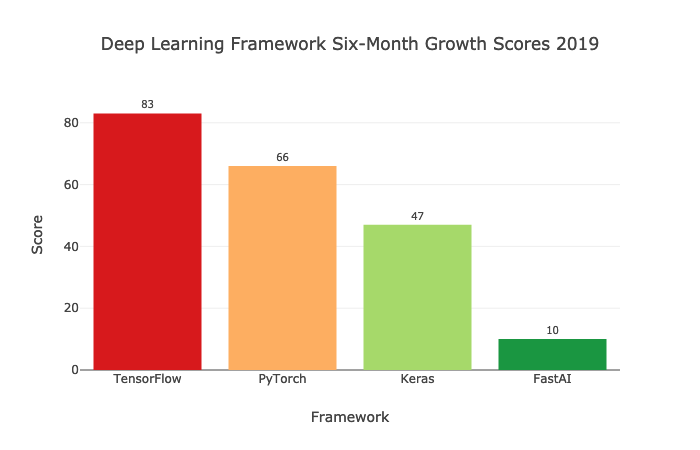
\includegraphics[width=.9\linewidth]{frameworks_2019.png}
	\end{column}%
\end{columns}
\vfill %

\vspace{2cm}
% \vfill % чёт не работает 

\scriptsize
\color{blue} \url{https://towardsdatascience.com/deep-learning-framework-power-scores-2018-23607ddf297a} \\
\url{https://keras.io/why-use-keras/}
\end{frame} 


\begin{frame}{Tensorflow 2.0}
\begin{center}
	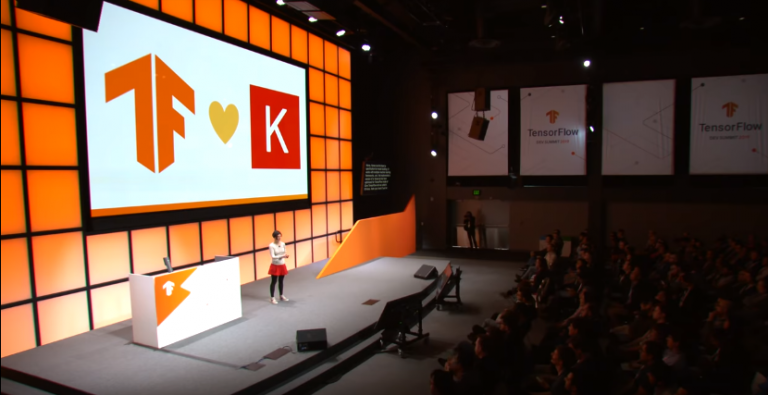
\includegraphics[width=.8\linewidth]{tf2.png}
\end{center}
\vfill %
\scriptsize
\color{blue} \url{https://www.tensorflow.org/beta/guide/effective_tf2}
\end{frame} 


\begin{frame}{Tensorflow 2.0}
\begin{center}
	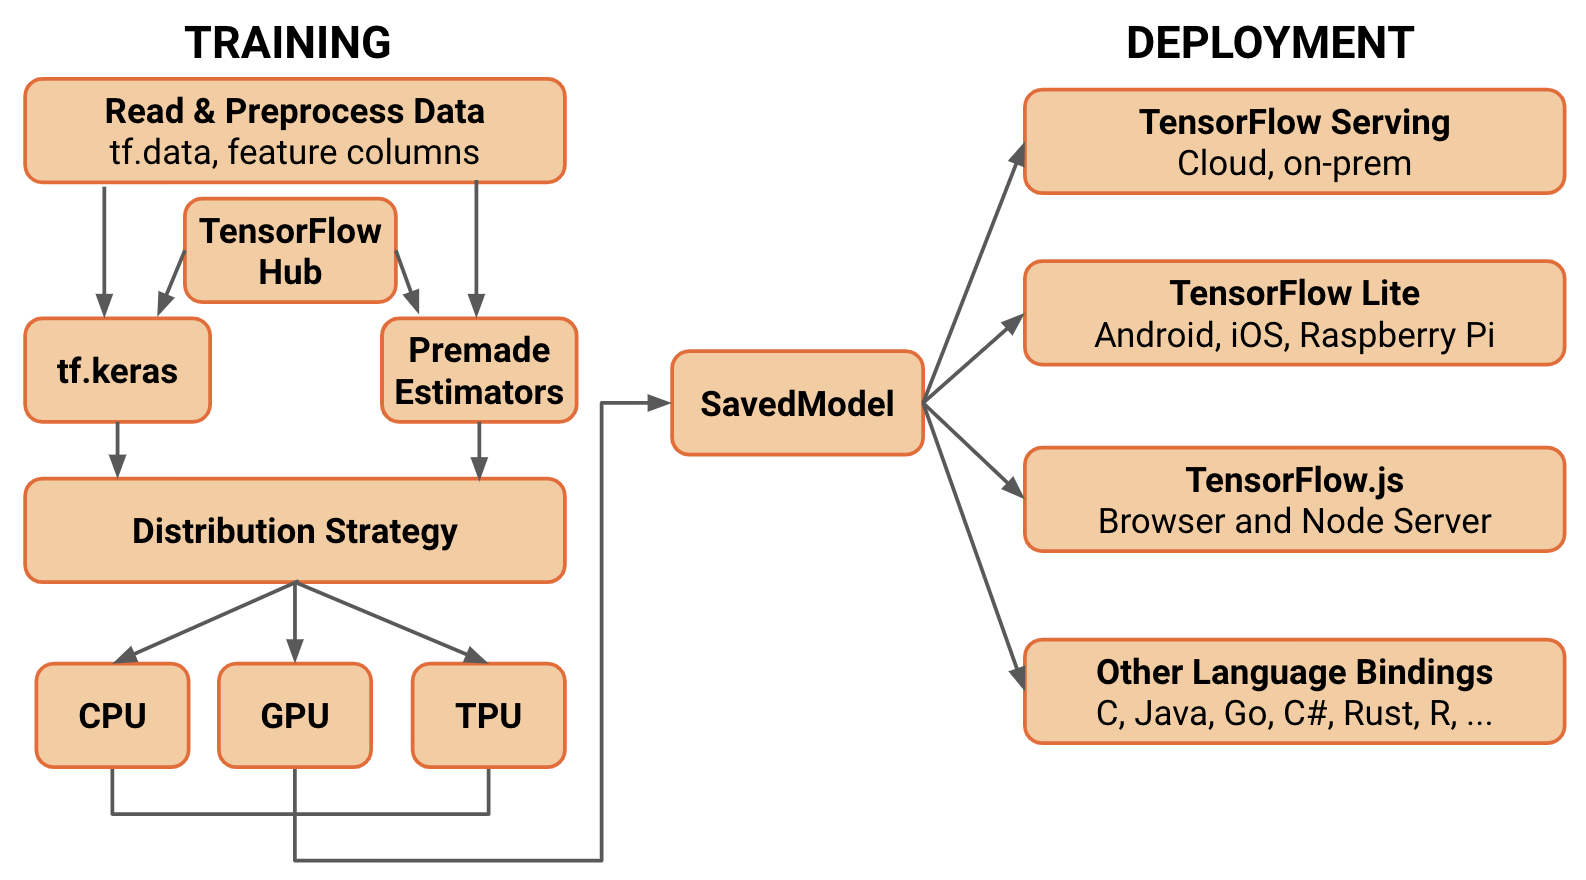
\includegraphics[width=.9\linewidth]{tensorflow_Str.png}
\end{center}
\end{frame} 


\begin{transitionframe}
	\begin{center}
		\Huge Немного истории
	\end{center}
\centering \href{https://vk.com/skialz}{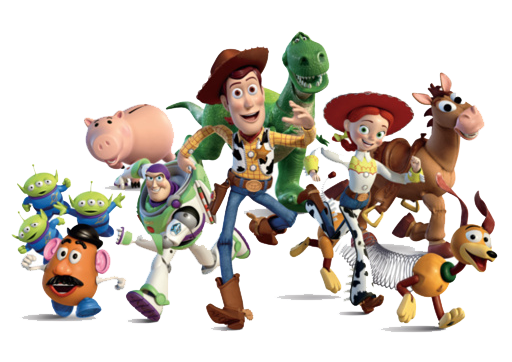
\includegraphics[scale = 0.25]{story.png}}
\end{transitionframe}

%%%%%%%%%%%%%%%%%%%%%%%%%%%
%%%%%% Реальные события 
%%%%%%%%%%%%%%%%%%%%%%%%%%%

{
	\usebackgroundtemplate{ 
		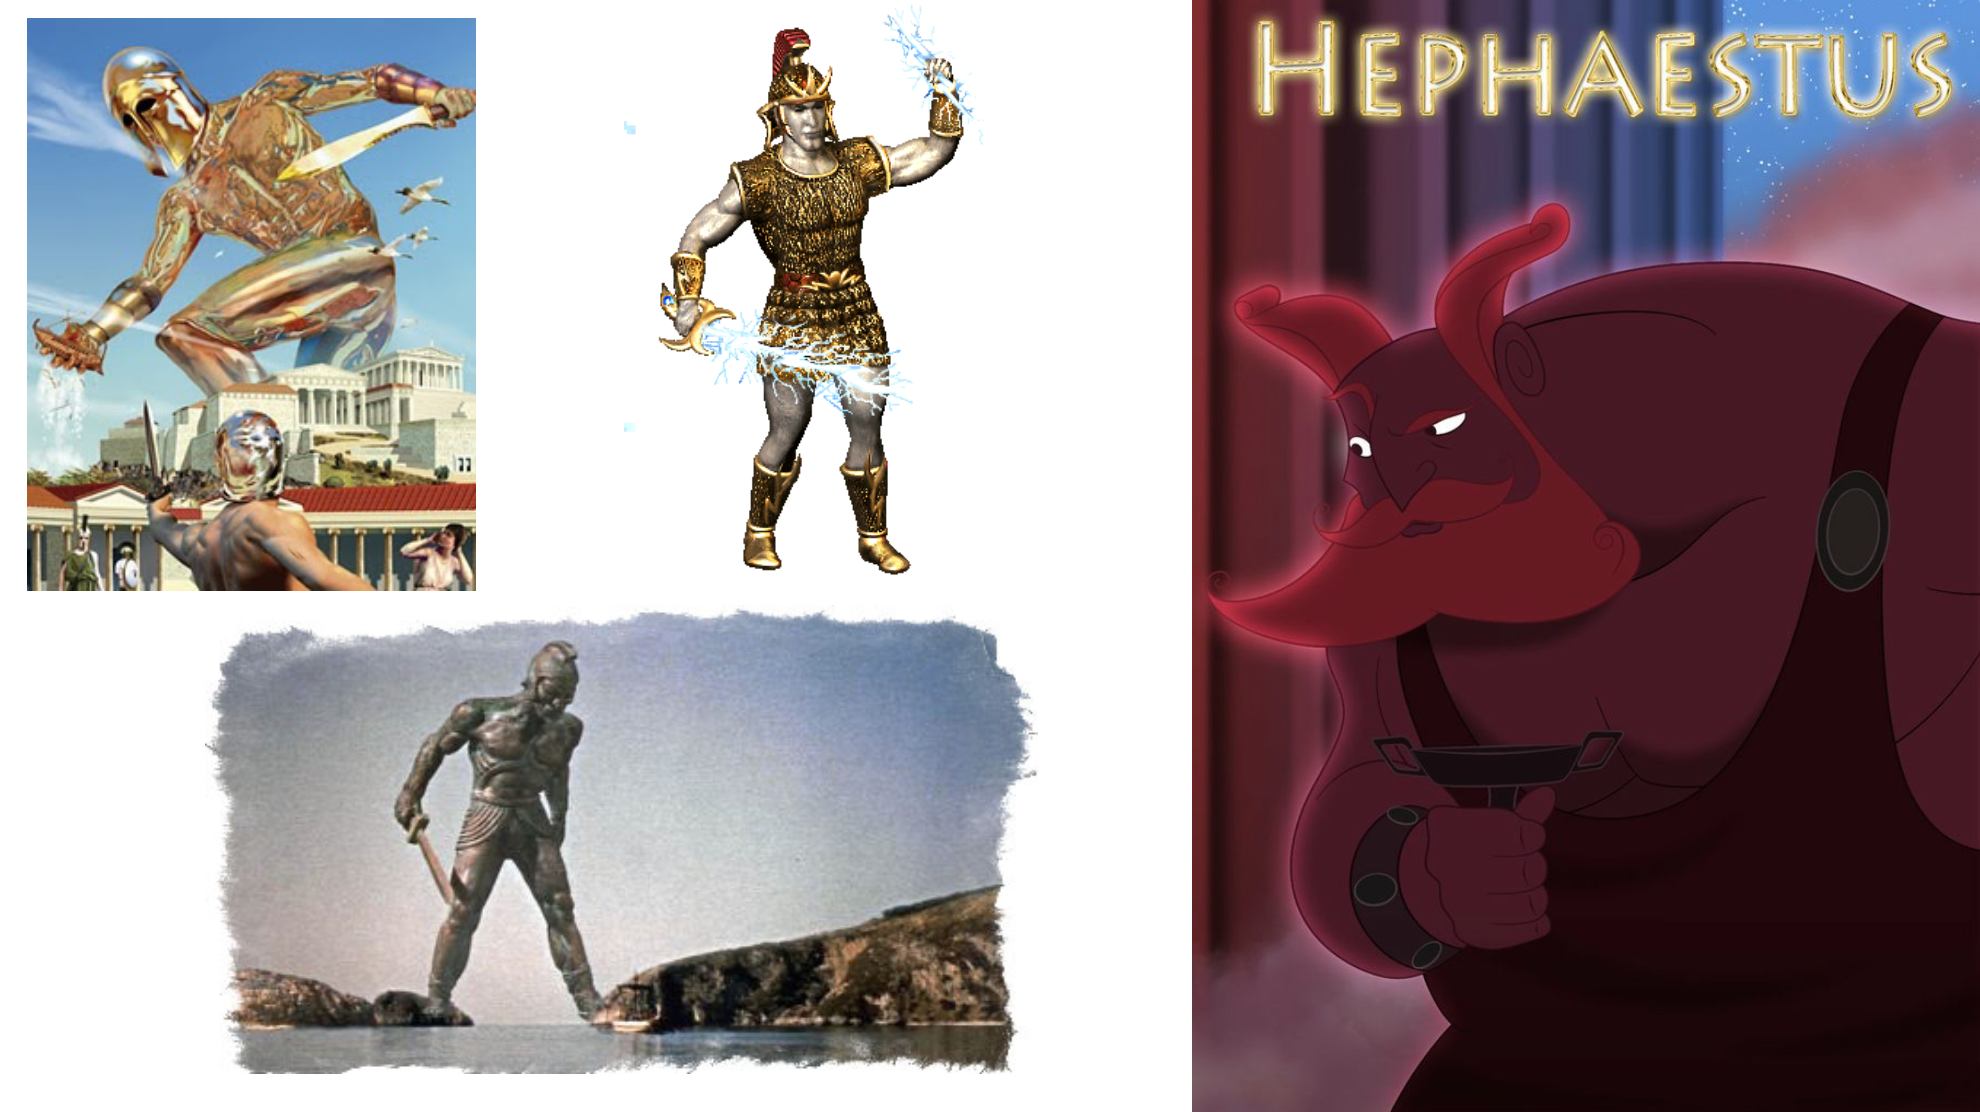
\includegraphics[width=\paperwidth]{history_1.png}}
	\begin{frame}
\end{frame}
}

{
\usebackgroundtemplate{ 
	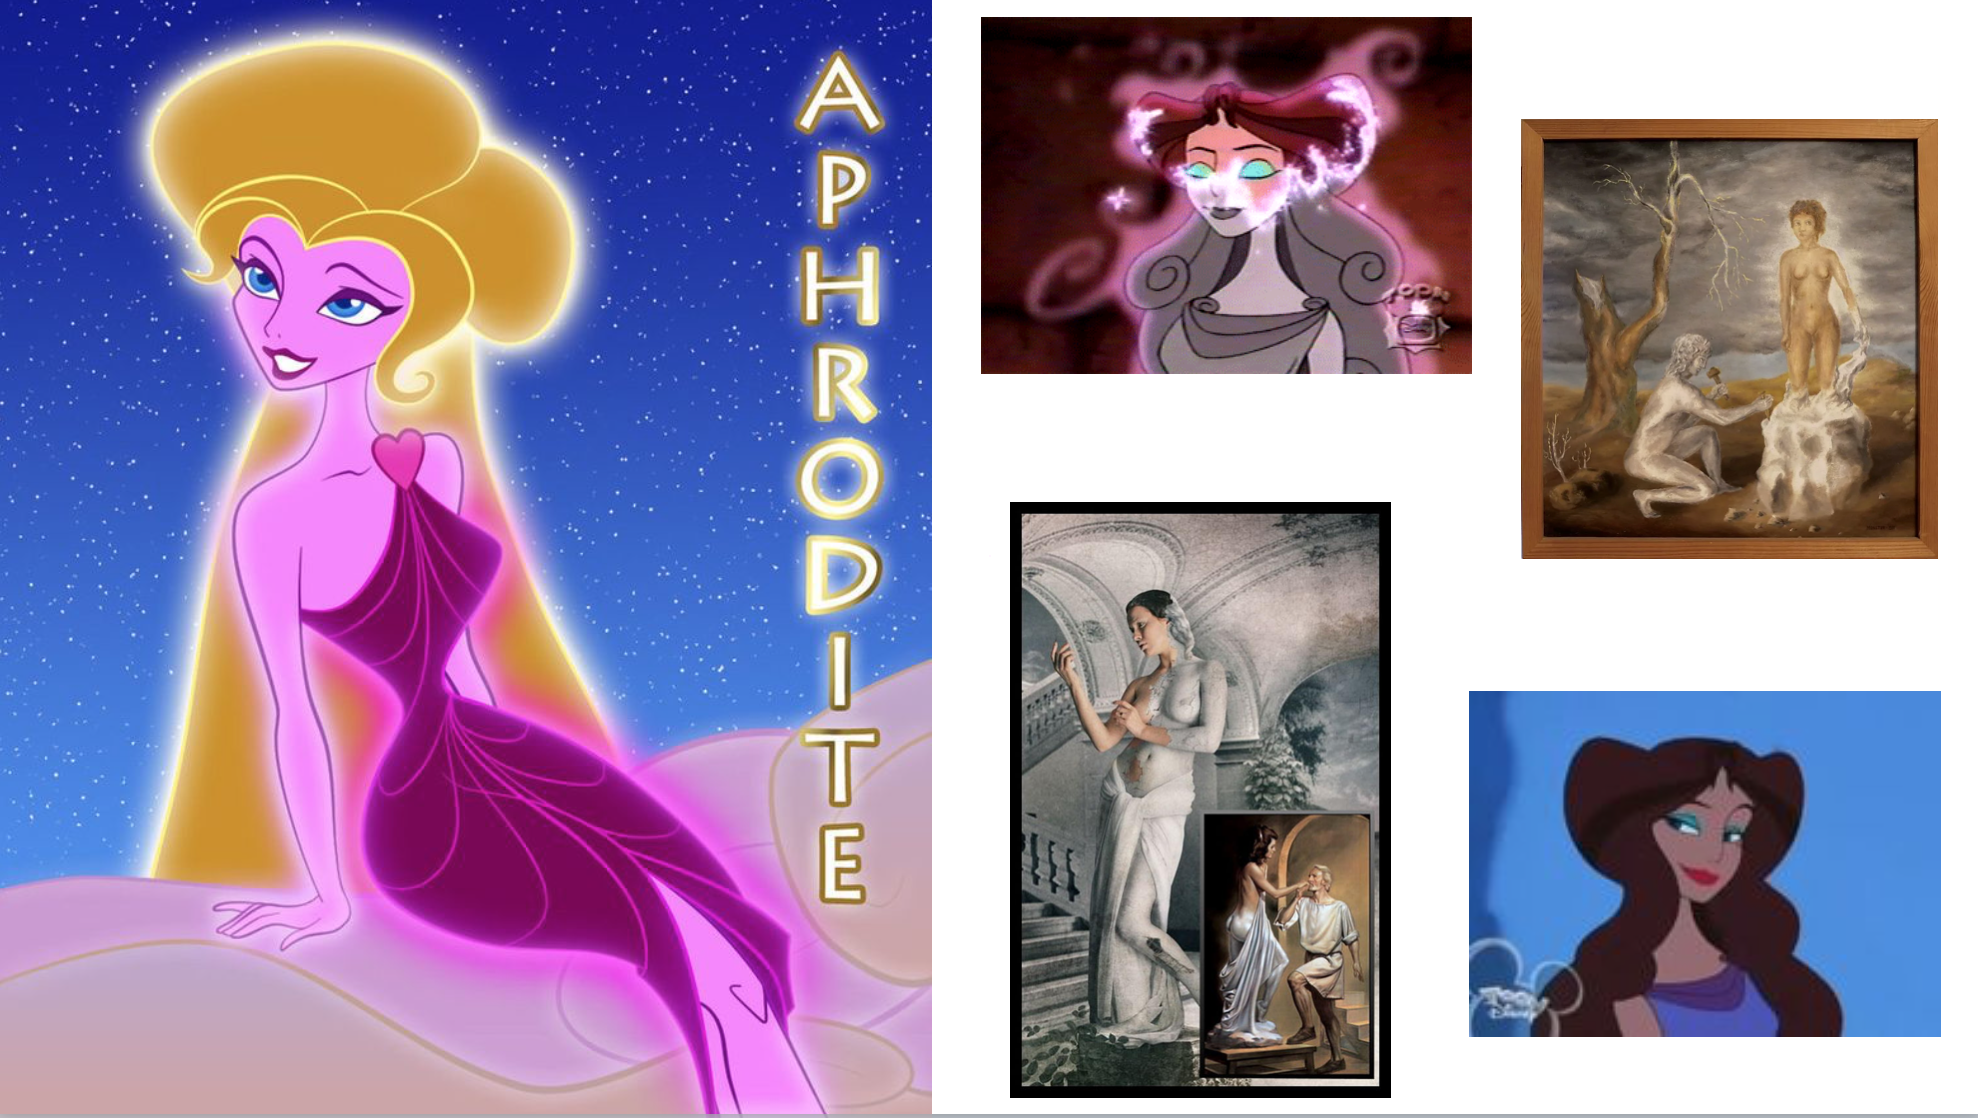
\includegraphics[width=\paperwidth]{history_2.png}}
\begin{frame}
\end{frame}
}

{
\usebackgroundtemplate{ 
\includegraphics[width=\paperwidth]{history_3.png}}
\begin{frame}
\end{frame}
}

{
\usebackgroundtemplate{ 
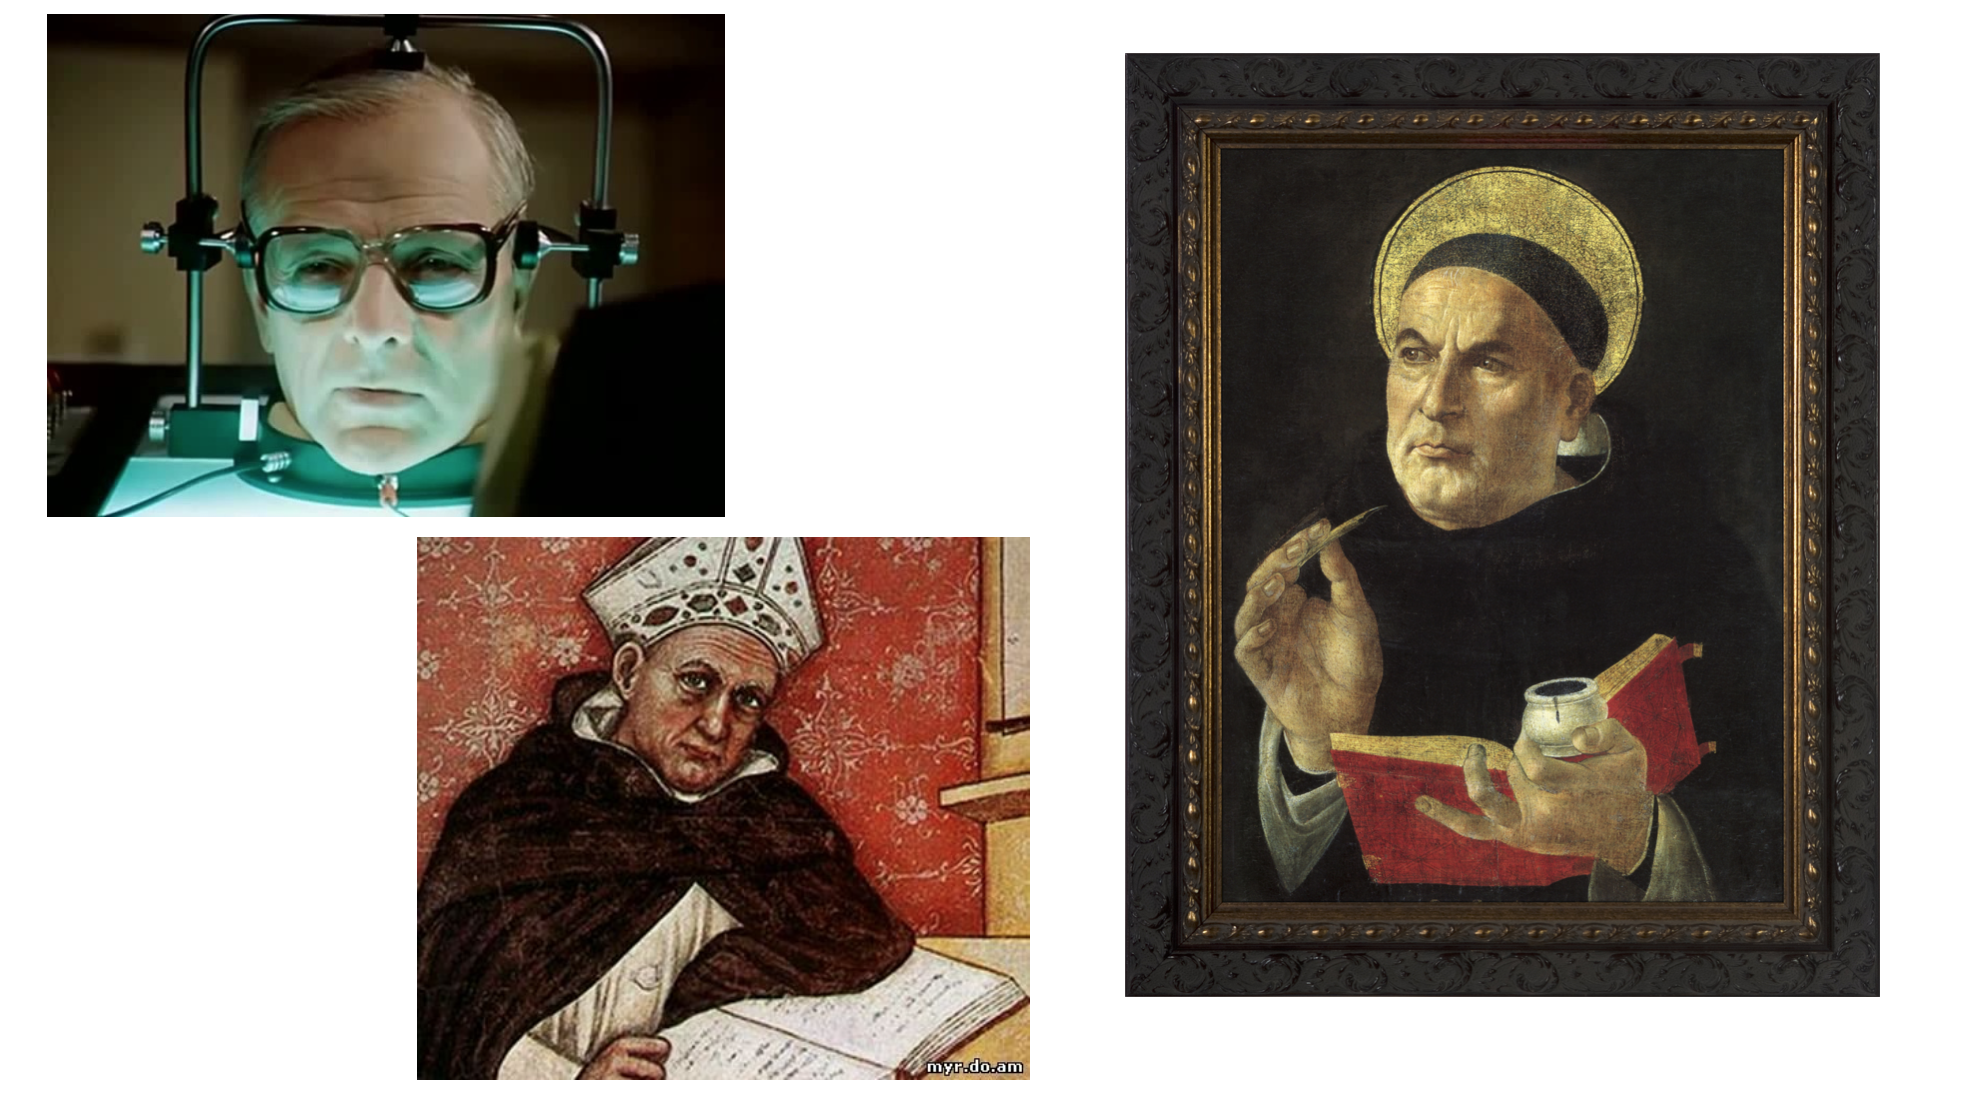
\includegraphics[width=\paperwidth]{history_4.png}}
\begin{frame}
\end{frame}
}

{
\usebackgroundtemplate{ 
\includegraphics[width=\paperwidth]{history_5.png}}
\begin{frame}
\end{frame}
}

{
\usebackgroundtemplate{ 
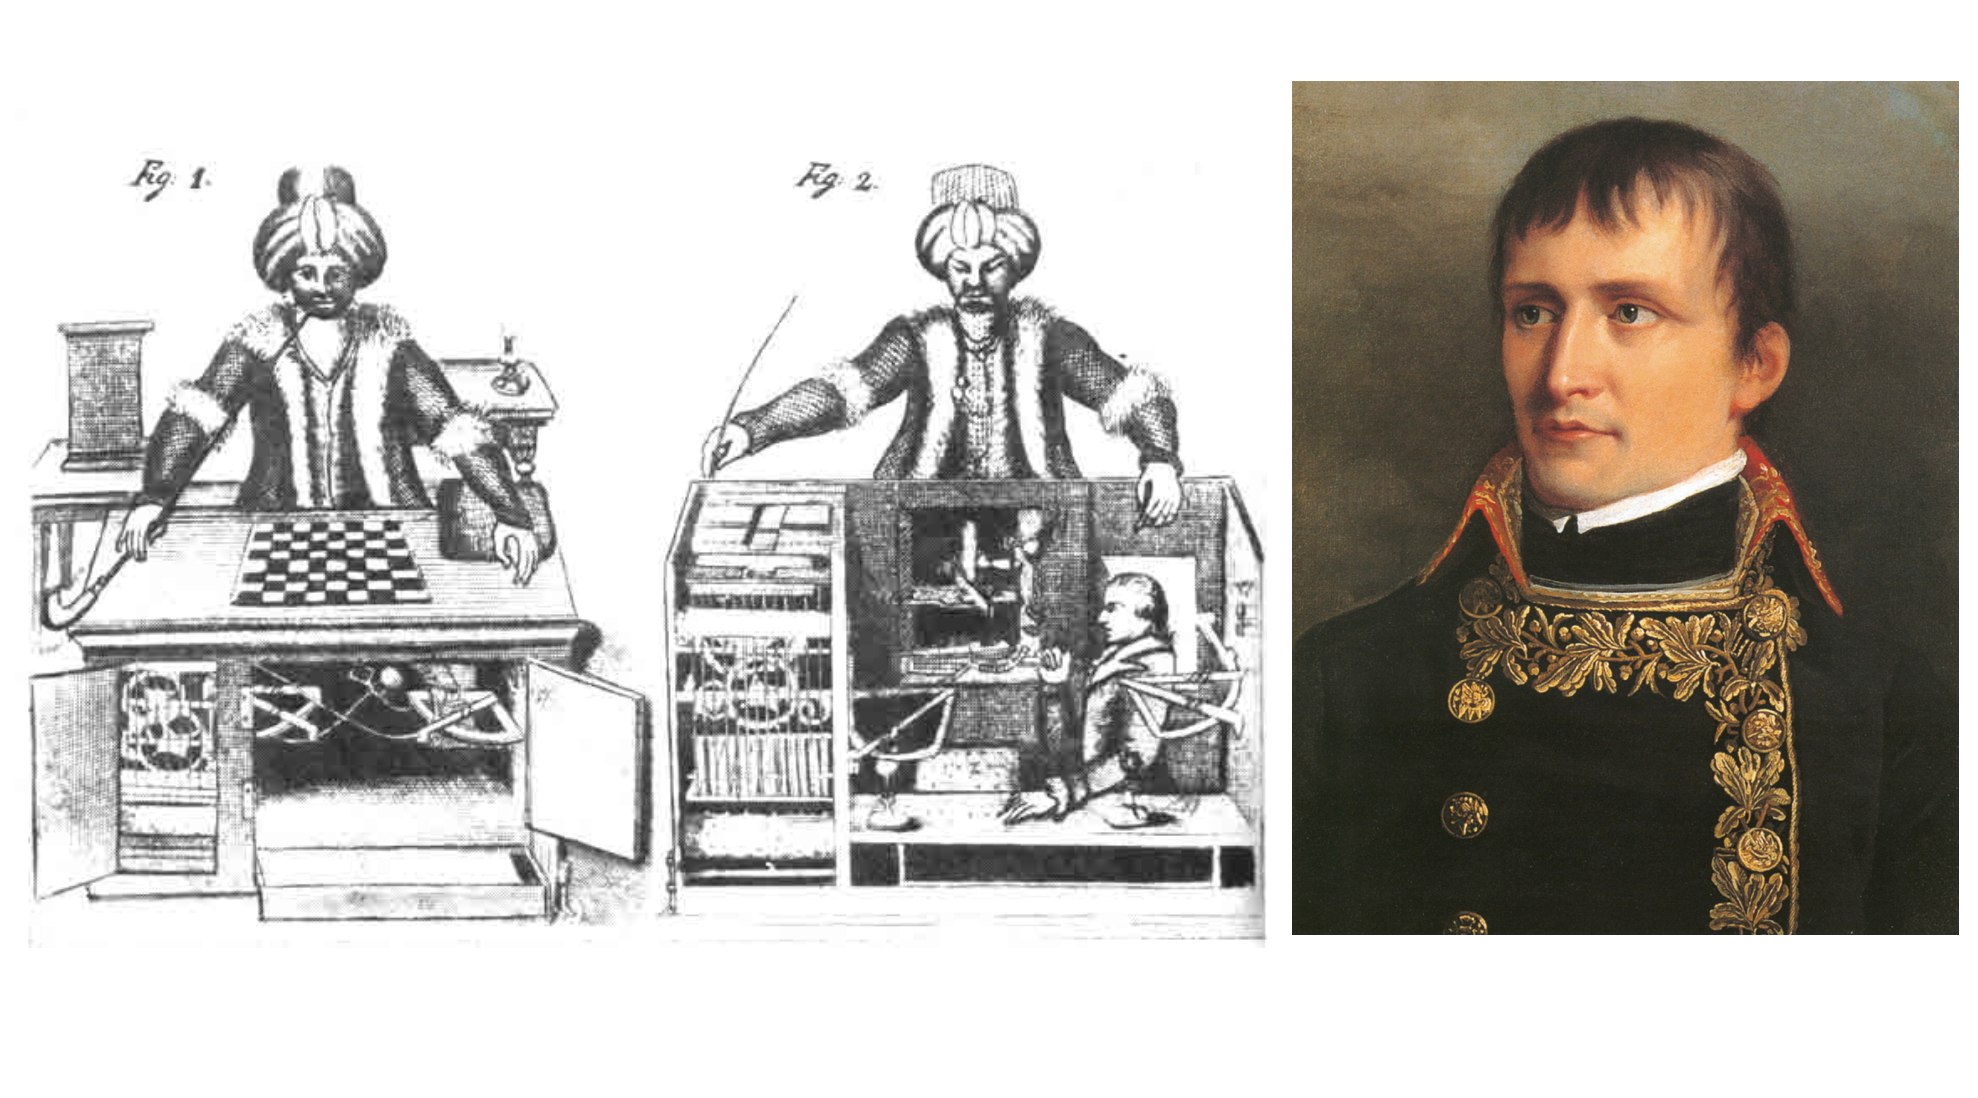
\includegraphics[width=\paperwidth]{history_6.png}}
\begin{frame}
\end{frame}
}

%%%%%%%%%%%%%%%%%%%%%%%%%%%%%%%
%%%%%% Дальше вымышленные события
%%%%%%%%%%%%%%%%%%%%%%%%%%%%%%%

\begin{frame}{Первый формальный нейрон (1943)}
\begin{columns}[T] % align columns
	\begin{column}{.48\textwidth}
		\centering 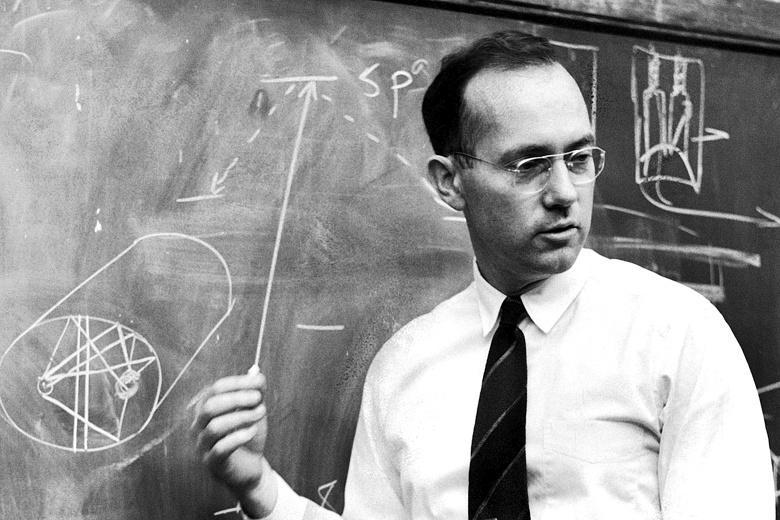
\includegraphics[scale=0.2]{pitts.jpg}\\
		\mbox{ } \\
		\color{blue} Уолтер Питтс
	\end{column}%
	\hfill%
	\begin{column}{.48\textwidth}
		\centering 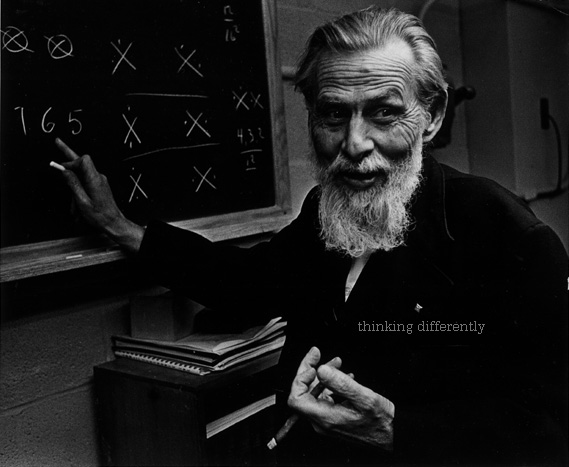
\includegraphics[scale=0.23]{makk.jpg}\\
		\mbox{ } \\
		\color{blue}  Уоррен Маккалок
	\end{column}%
\end{columns}
\end{frame}


\begin{frame}{Первый формальный нейрон (1958)}
\begin{columns}[T] % align columns
	\begin{column}{.33\textwidth}
		\centering 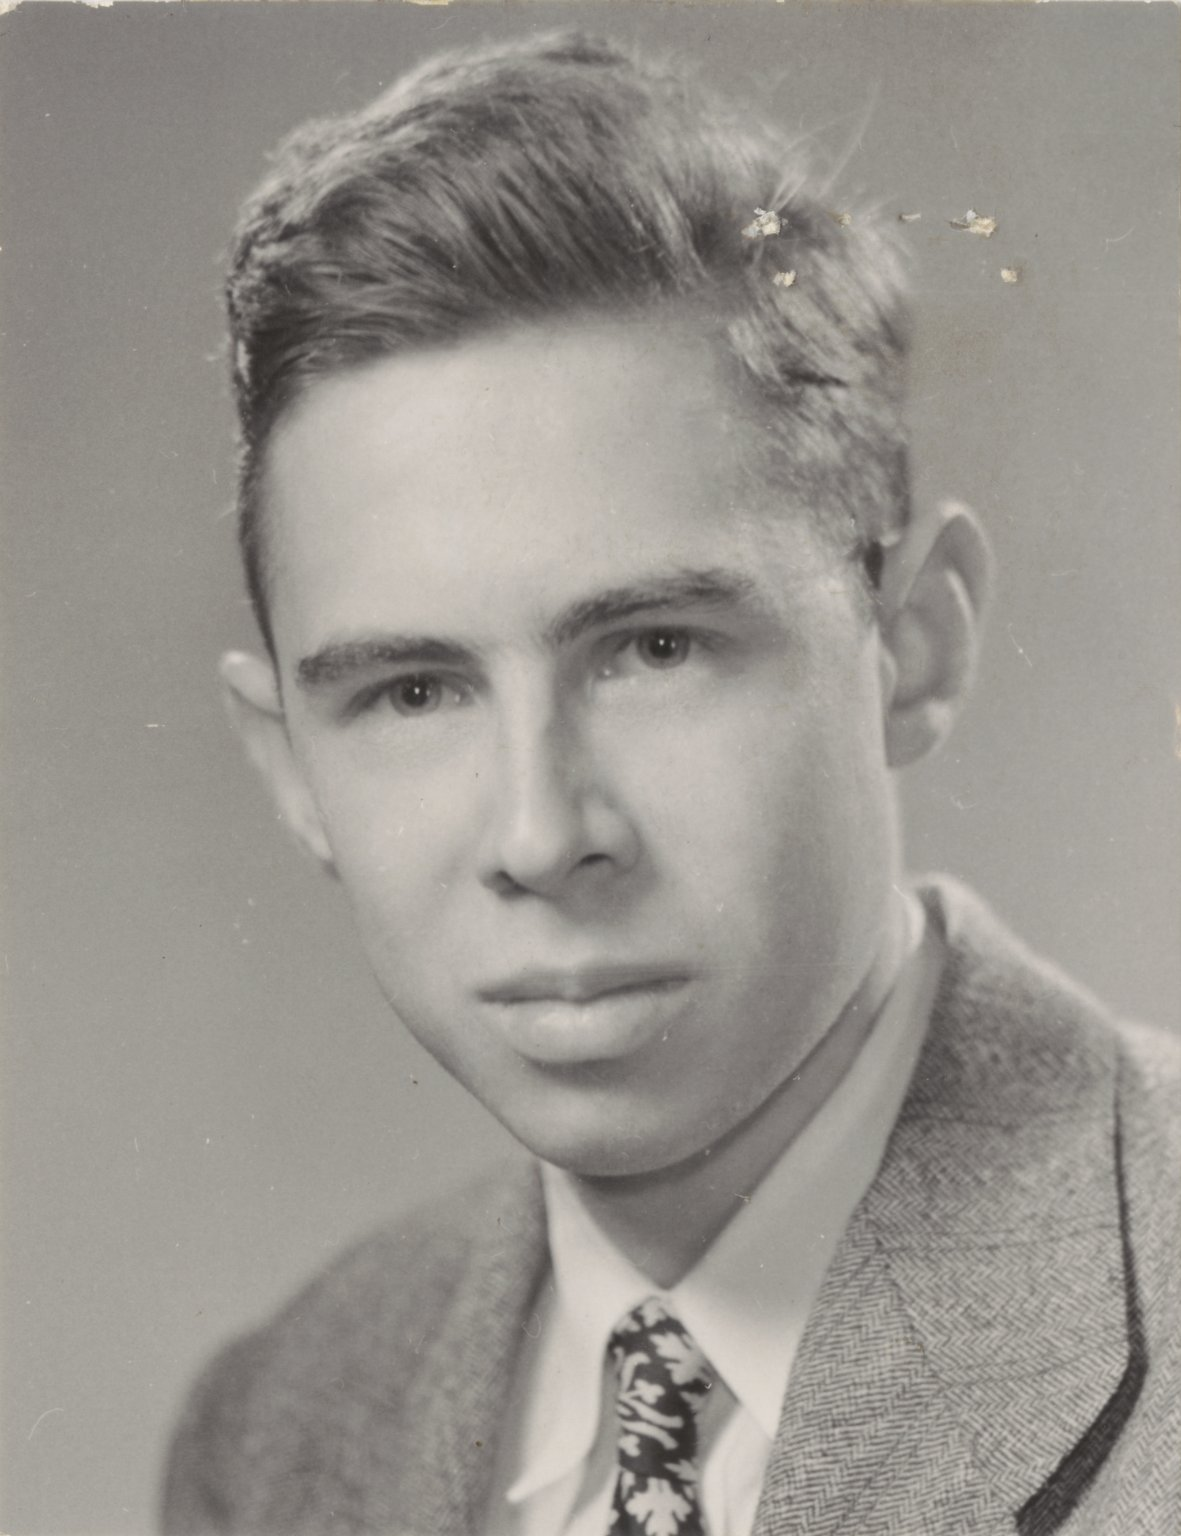
\includegraphics[scale=0.1]{rozen.jpg}\\
		\mbox{ } \\
		\color{blue} Фрэнк Розенблатт
	\end{column}%
	\hfill%
	\begin{column}{.33\textwidth}
		\centering 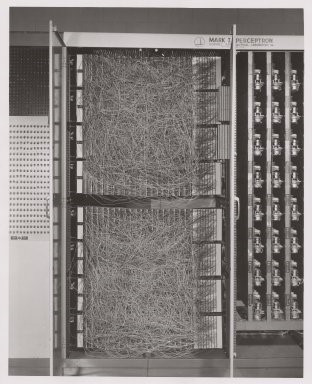
\includegraphics[scale=0.54]{rozen_mark2.jpg}\\
		\mbox{ } \\
		\color{blue}  Mark I Perceptron \\ (Компуктер Розенблата)
	\end{column}%
	\hfill%
	\begin{column}{.33\textwidth}
		\centering 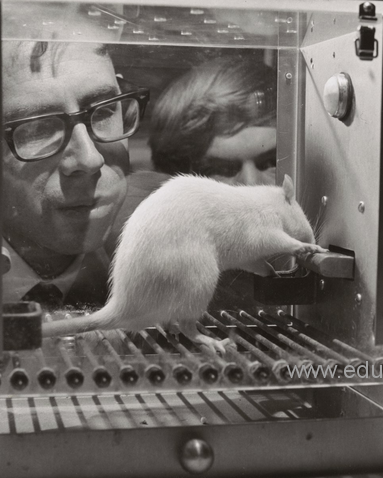
\includegraphics[scale=0.325]{rozen_mouse.png}\\
		\mbox{ } \\
		\color{blue}  Гарольд \\ (Мышь Розенблатта)
	\end{column}%
\end{columns}
\end{frame}


\begin{frame}{Дартмундский семинар (1956)}
\begin{columns}[T] % align columns
	\begin{column}{.48\textwidth}
		\centering \color{blue} Марвин Минский
		 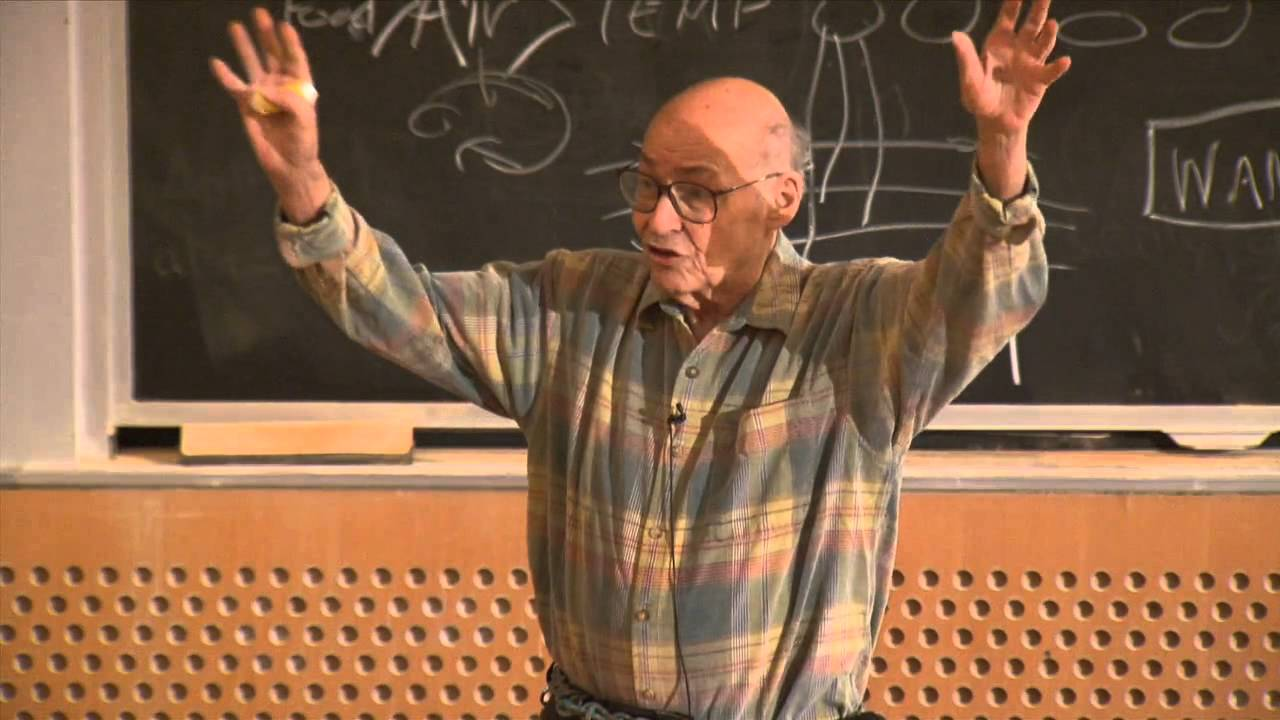
\includegraphics[scale=0.1]{minski.jpg}\\
		 \mbox{ } \\
		 \color{blue} Натаниэль Рочестер \\
		 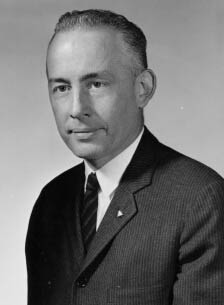
\includegraphics[scale=0.33]{rochester.jpeg}\\
	\end{column}%
	\hfill%
	\begin{column}{.48\textwidth}
		\centering 		 \color{blue} Джон Маккарти
		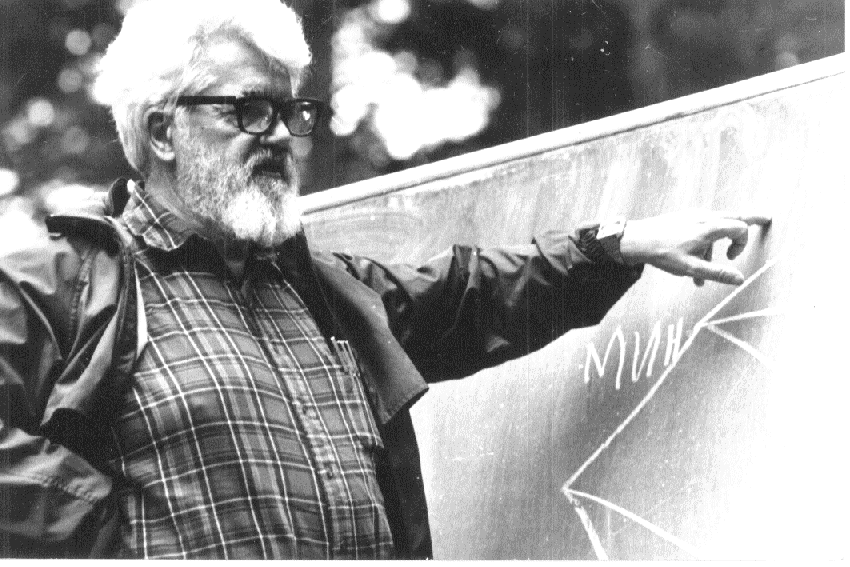
\includegraphics[scale=0.14]{makart.png}\\
		\mbox{} \\		
		 \color{blue} Клод Шеннон \\
		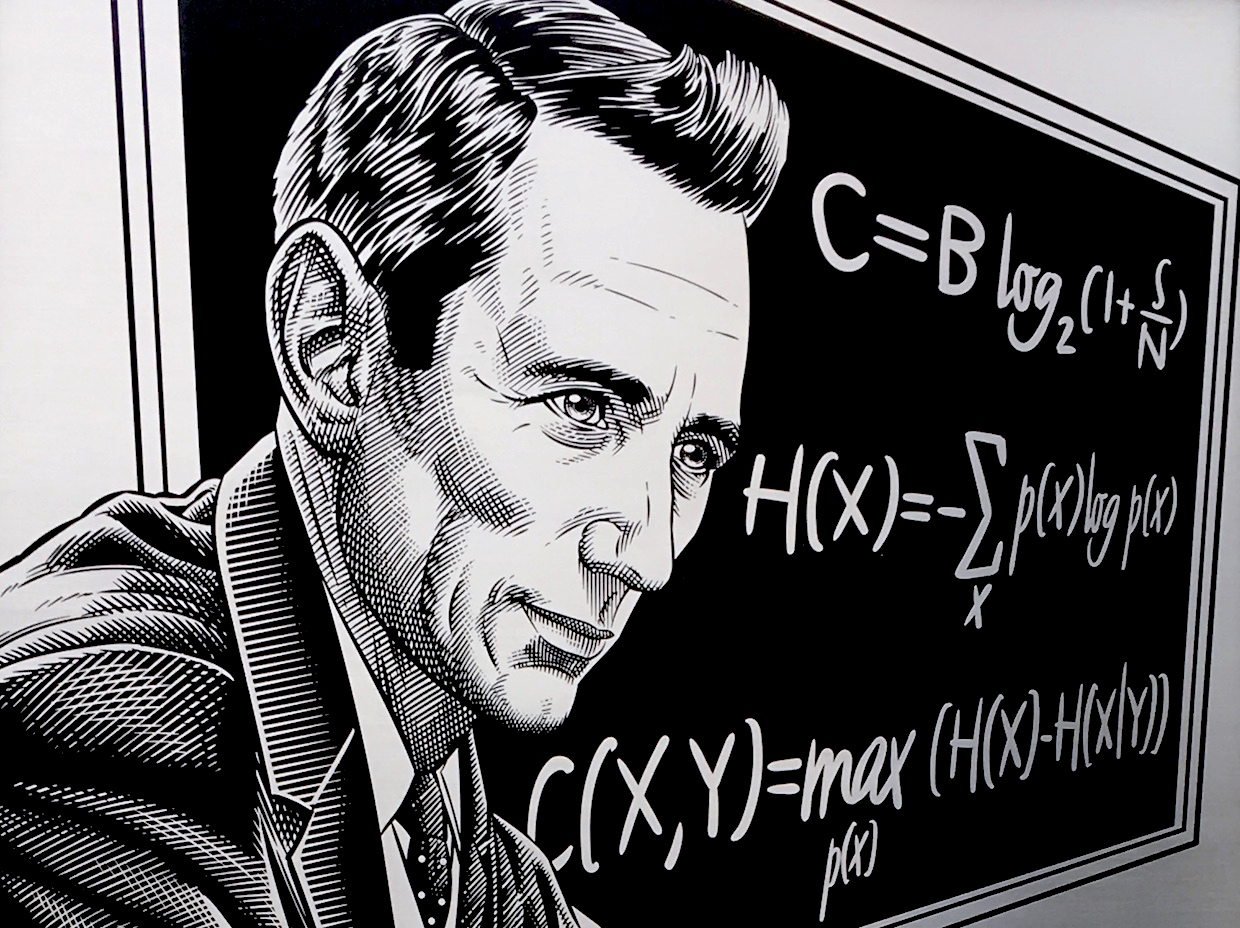
\includegraphics[scale=0.1]{shennon.jpeg}\\
	\end{column}%
\end{columns}
\end{frame}

{
\usebackgroundtemplate{ 
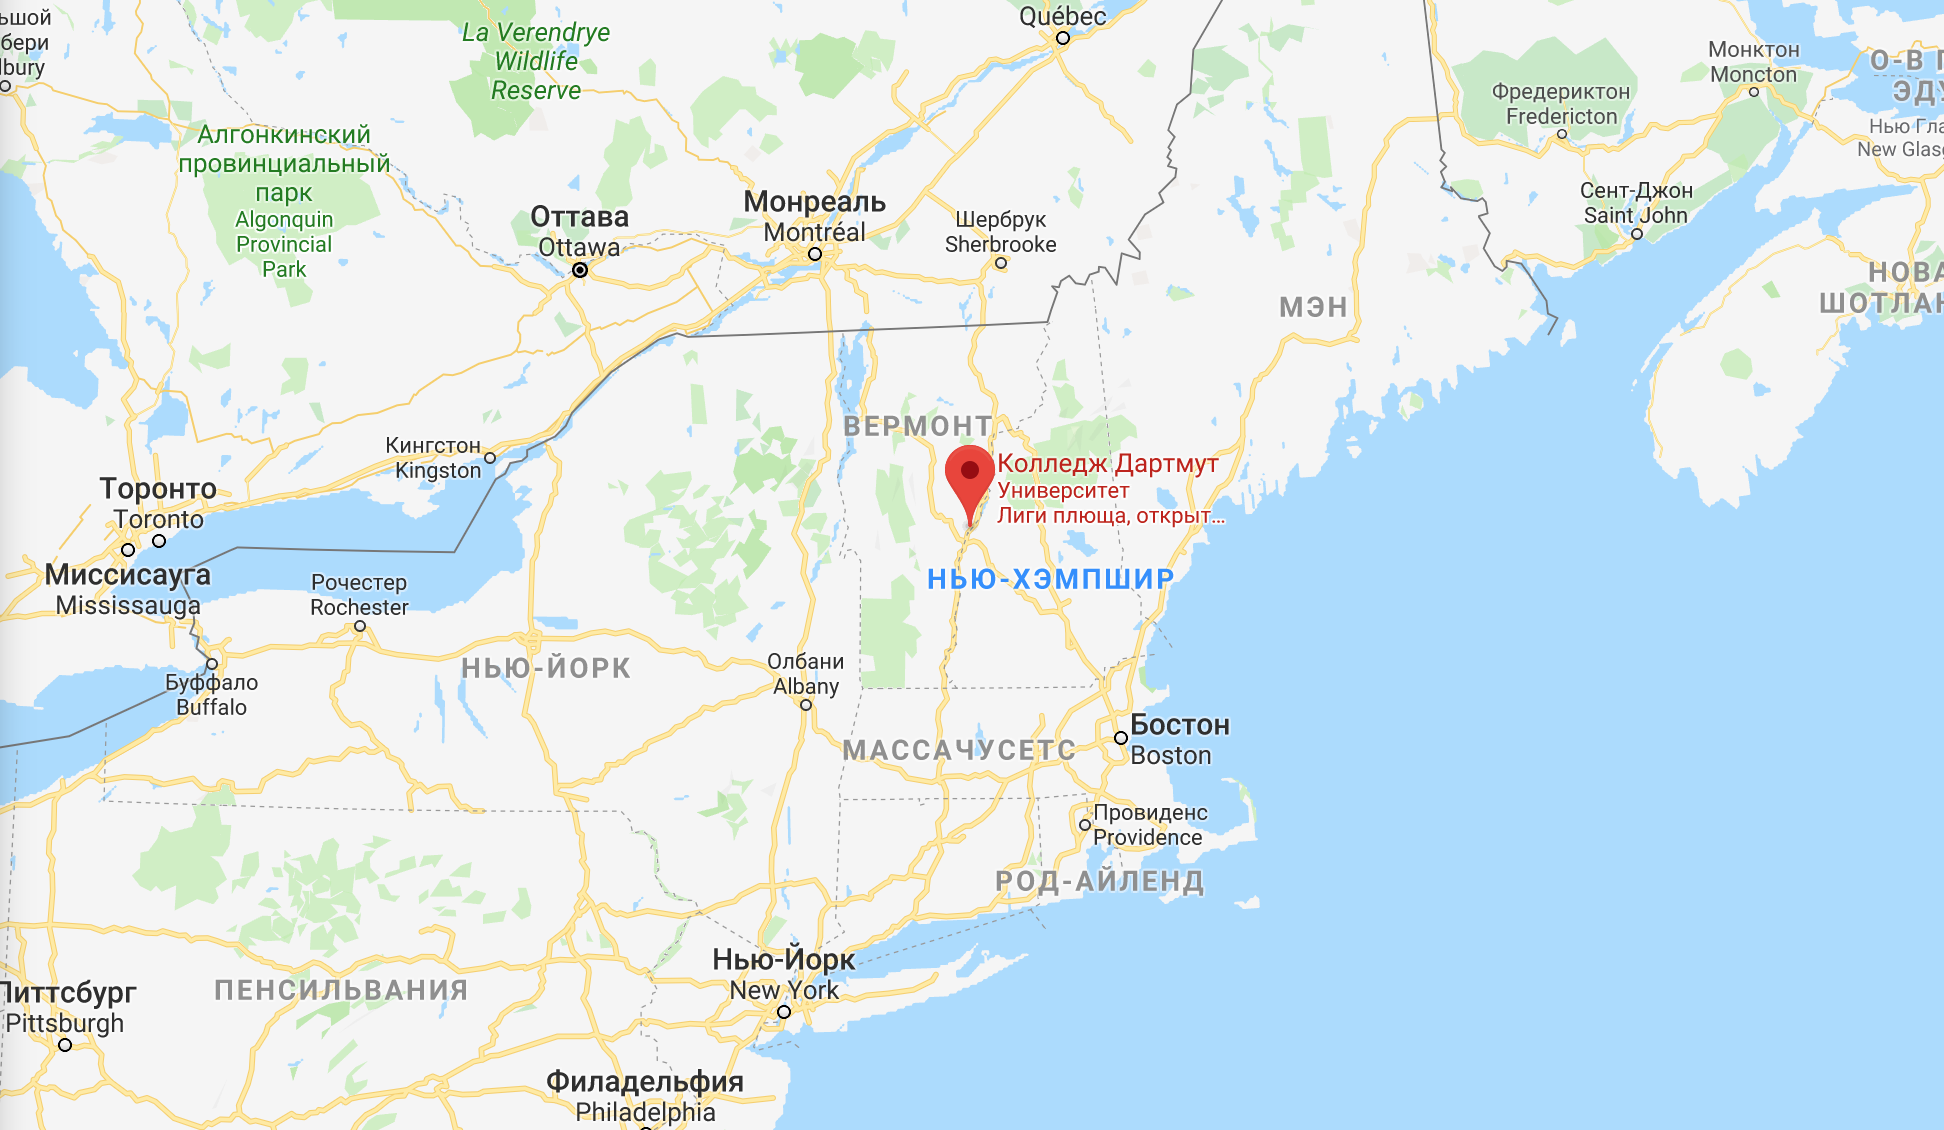
\includegraphics[width=\paperwidth]{dartmut.png}}
\begin{frame}
\end{frame}
}


\begin{frame}{Зима близко}
	\begin{columns}[T]%
		\begin{column}{.55\textwidth}%
		\begin{wideitemize} 
		\item 1956 — Дартмунтский семинар, море оптимизма
		
		\item 1958 — Персептрон Розенблатта
		
		\item середина 1960-х — провал крупного проекта по машинному переводу с русского на английский и наоборот 
		
		\item 1969 — Марвин Минский и Сеймур Пейперт опубликовали книгу «Персептроны» с критикой 
		
		\end{wideitemize} 
		\end{column}%
		\hfill%
		\begin{column}{.45\textwidth}
		\begin{center}
		
\includegraphics[width=.99\linewidth]{stark.jpg}
		\end{center}
		\end{column}%
	\end{columns}%
\end{frame}


\begin{frame}{Зима наступила}
\begin{columns}[T]%
	\begin{column}{.7\textwidth}%
		\begin{wideitemize} 
			\item \alert{Зима искуственного интеллекта} — период в истории исследований искусственного интеллекта, связанный с сокращением финансирования и  снижением интереса
			
			\item  Две длительные «зимы» относят к периодам 1974—1980 годов и 1987—1993 годов
			
			\item Несмотря на спад финансирования, исследования продолжались		
		\end{wideitemize} 
	\end{column}%
	\hfill%
	\begin{column}{.3\textwidth}%
		\begin{center}
			
\includegraphics[width=.99\linewidth]{stark_2.png}
		\end{center}
	\end{column}%
\end{columns}%
\end{frame}


\begin{frame}{Оттепель}
	\begin{wideitemize} 
		\item 1970-е — Расцвет экспертных систем, принимающих решения на основе большого числа правил и знаний о предметной области 
		
		\item {\color{blue} \href{https://en.wikipedia.org/wiki/Mycin}{MYCIN}} накопила около $600$ правил для идентификации вирусных бактерий и выдачи подходящего метода лечения (угадывала в $69\%$ случаев, лучше любого начинающего врача)
		
		\item 1980-е  — появилось много разных архитектур
		
		\item 1980-е — алгоритм обратного распространения ошибки (backpropagation) позволил обучать сети за линейное время
		
		\item Ренессанс нейронных сетей 
	\end{wideitemize} 
\end{frame}


\begin{frame}{Зима близко}
	\begin{columns}[T] 
		\begin{column}{.6\textwidth}
			\begin{wideitemize} 
				\item Новая волна оптимизма
				
				\item 1986 — один из первых AI-отделов экономил компании DEC около 10 миллионов долларов в год
				
				\item Завышенные ожидания снова лопнули
				
				\item 1990-е — ударными темпами развивается классическое машинное обучение
			\end{wideitemize} 
		\end{column}%
		\hfill%
		\begin{column}{.4\textwidth}
			\begin{center}
			
\includegraphics[width=.99\linewidth]{stark.jpg}
			\end{center}
		\end{column}%
	\end{columns}
\end{frame}


\begin{frame}{Революция (2005-2006)}
\begin{columns}[T] % align columns
	\begin{column}{.48\textwidth}
		\centering 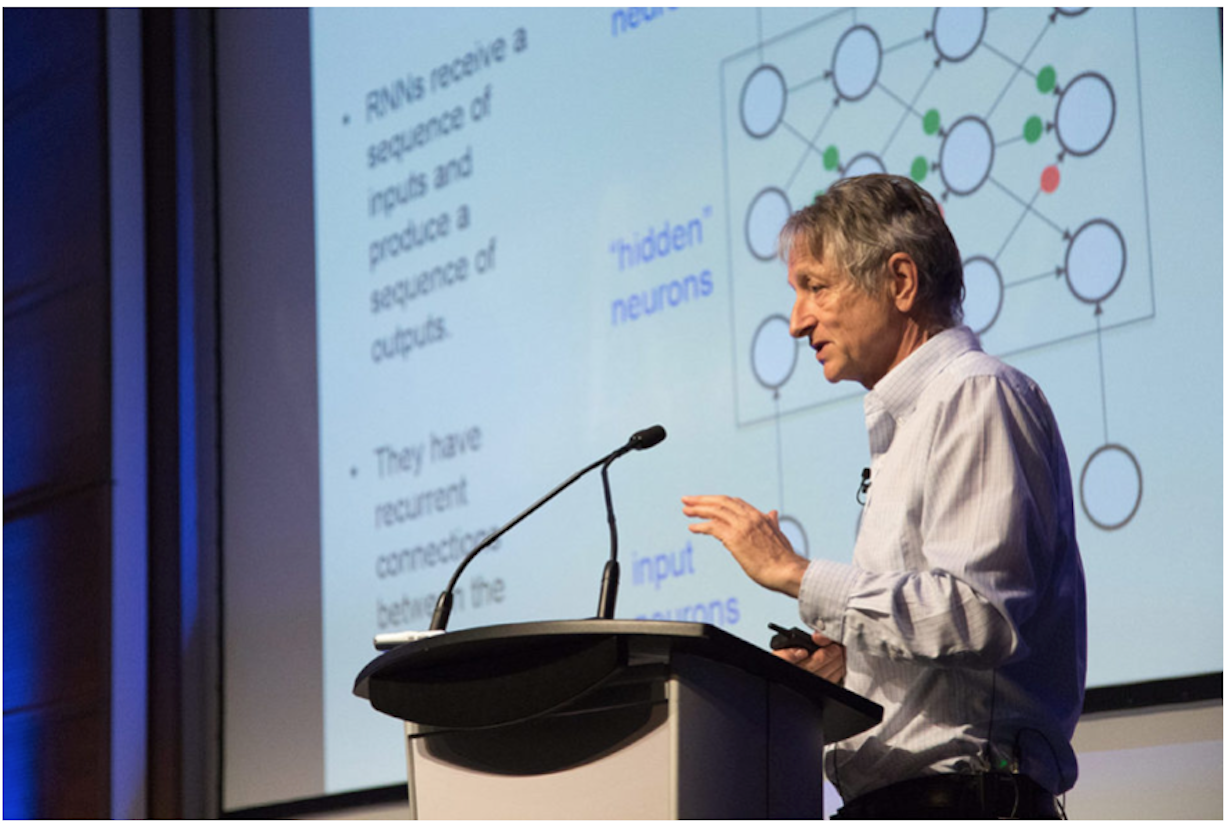
\includegraphics[scale=0.16]{hinton.png}\\
		\mbox{ } \\
		\color{blue} Джеффри Xинтон \\
		\small (университет Торонто)
	\end{column}%
	\hfill%
	\begin{column}{.48\textwidth}
		\centering 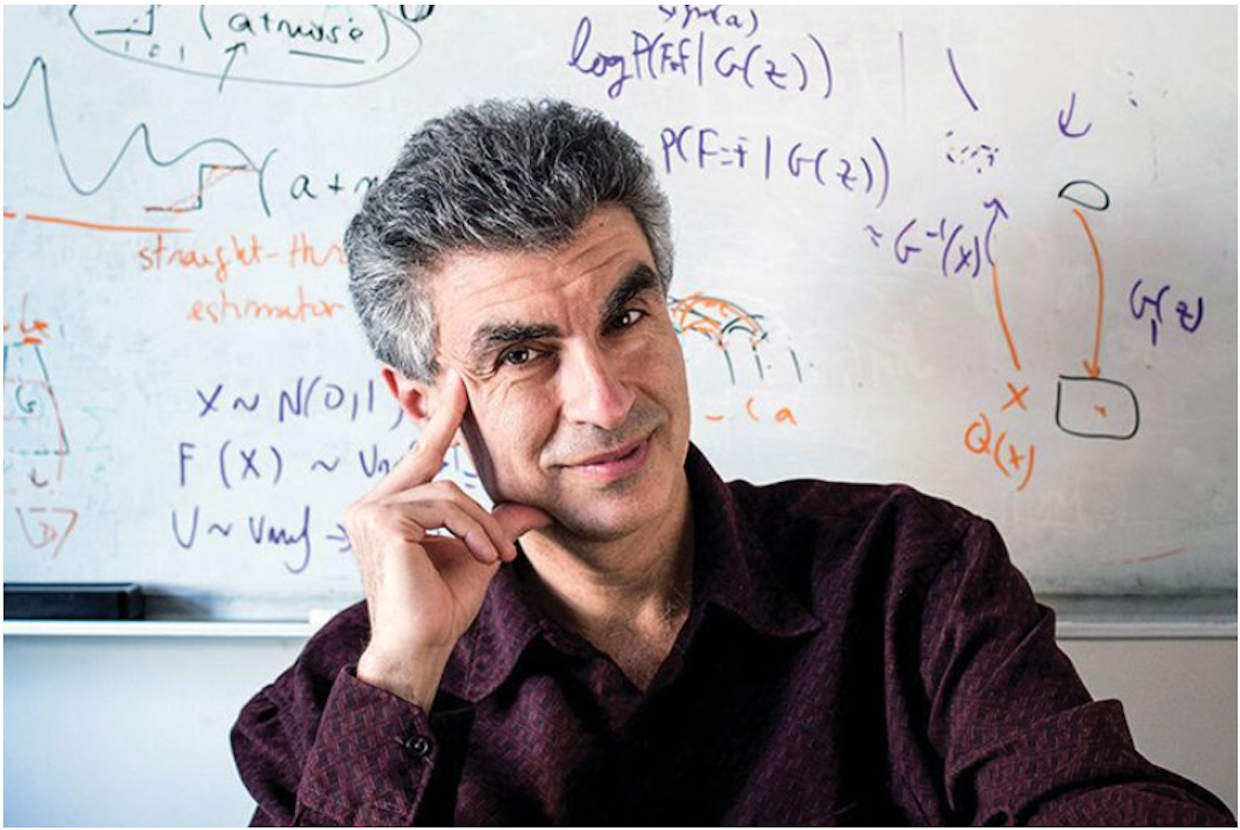
\includegraphics[scale=0.16]{bendji.png}\\
		\mbox{ } \\
		\color{blue}  Йошуа Бенджи \\
		\small (университет Монреаля)
	\end{column}%
\end{columns}
\end{frame}

\begin{frame}{Революция}
	\begin{wideitemize} 
		\item 2005-2006 — группы Хинтона и Бенджи научились обучать глубокие нейросетки
		
		\item Накопилось больше данных! Огромные данные! 
		
		\item Компьютеры стали на порядки мощнее! Появились крутые GPU! 
		
		\item На больших данных и мощностях заработали старые архитектуры
		
		\item Появились новые алгоритмы, эвристики и подходы
		
		\item Ящик Пандоры открыт! 
	\end{wideitemize} 
\end{frame}


{
\usebackgroundtemplate{ 
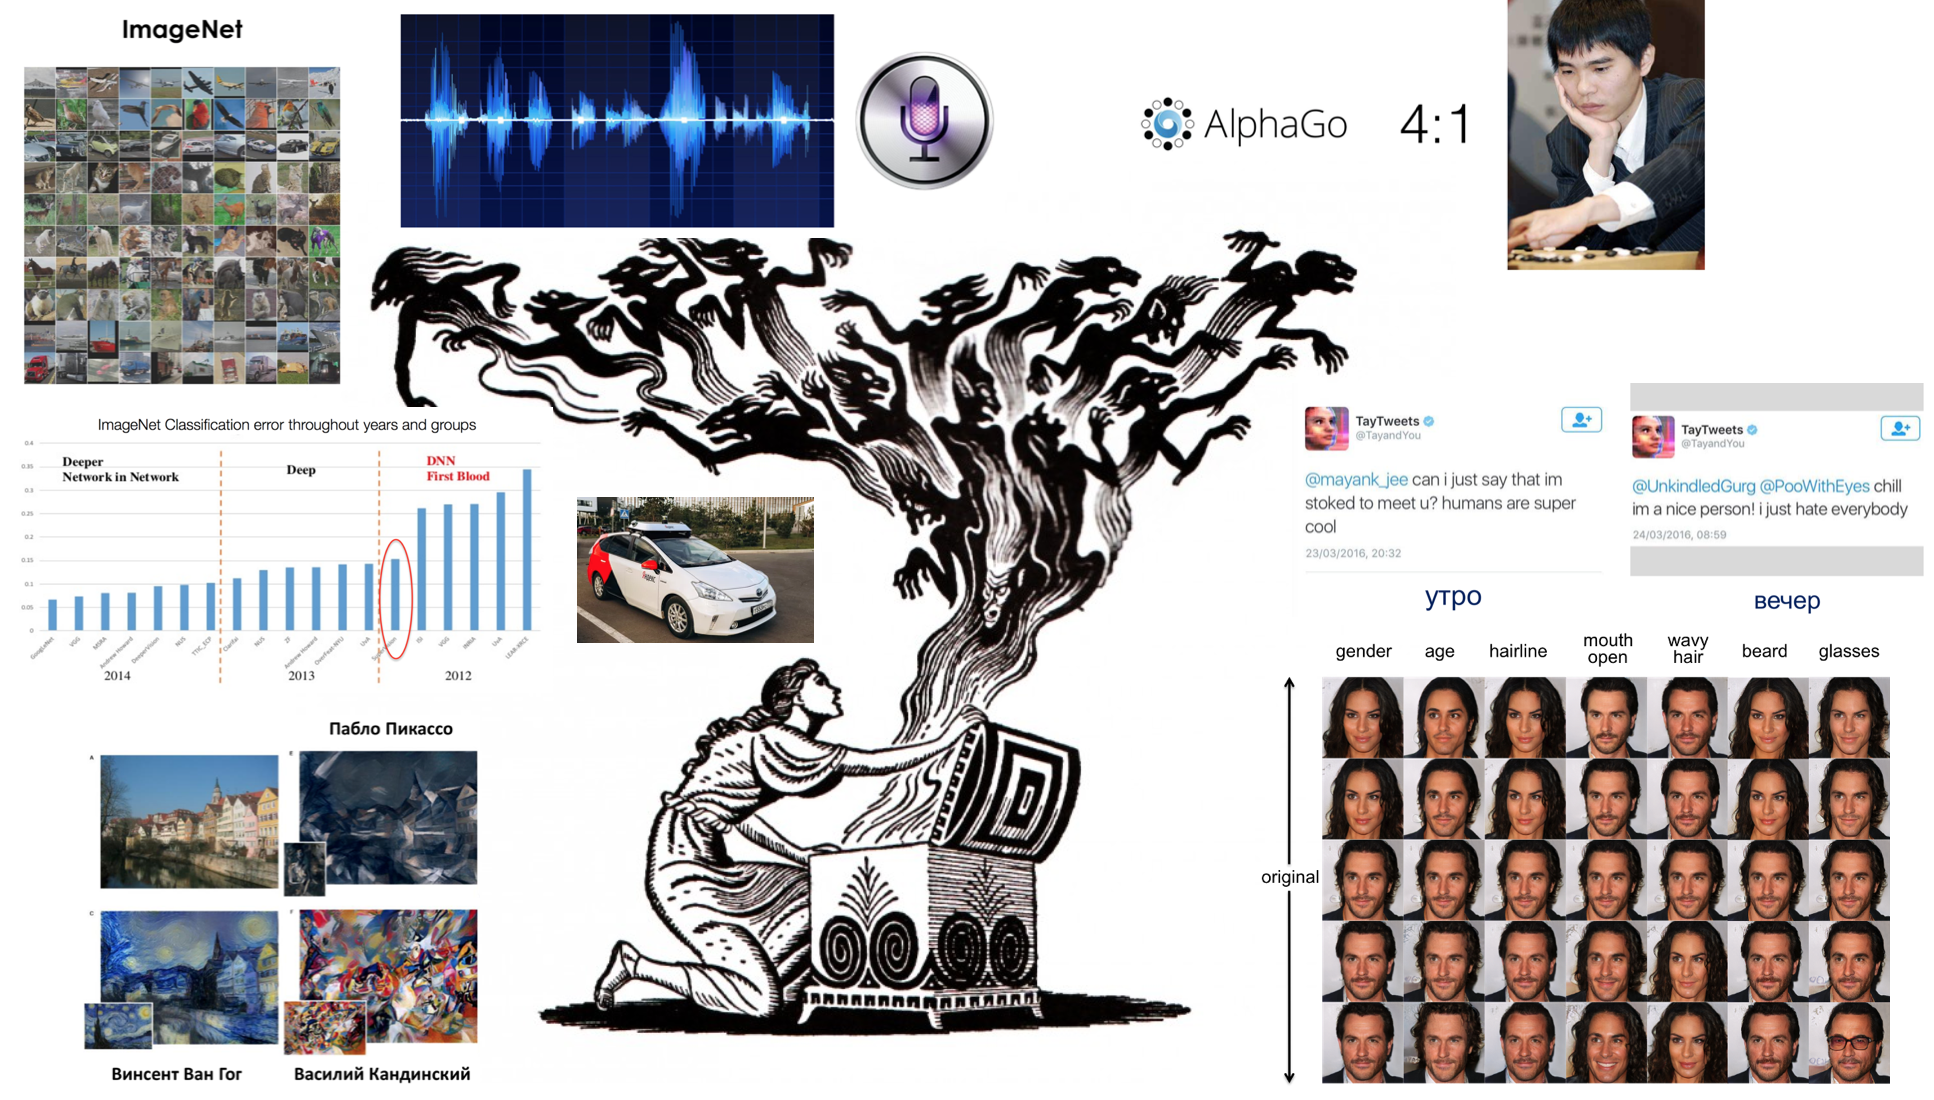
\includegraphics[width=\paperwidth]{pandora.png}}
\begin{frame}
\end{frame}
}


\begin{frame}{Новая зима близко  — ??? }
	\begin{center}
		
\includegraphics[width=.6\linewidth]{stark_3.jpeg}
	\end{center}
\end{frame}


\begin{frame}{или нет ... }
\begin{columns}
\begin{column}{0.6\textwidth}
	\begin{wideitemize}
		\item  Для того, чтобы сделать большое открытие нужно несколько гениев
		\item  Для того, чтобы внедрить его результаты нужна армия инженеров, которым не обязательно быть гениями
		\item  Мы сделали большое открытие и только начали повсюду его внедрять
		\item \alert{Пример:} изобретение электричества 
	\end{wideitemize}
\end{column}
\hfill%
\begin{column}{0.4\textwidth}
		\begin{center}
			
\includegraphics[width=.7\linewidth]{book_ch.jpg} \\
			\footnotesize Про будущее и Китай
		\end{center}
\end{column}
\end{columns}
\end{frame} 


\begin{transitionframe}
	\begin{center}
		\Huge Важные тренды
	\end{center}
\centering \href{https://vk.com/skialz}{
\includegraphics[scale = 0.15]{unicorn.png}}
\end{transitionframe}


\begin{frame}{\# 1. Точность сетей растёт}
\begin{center}
	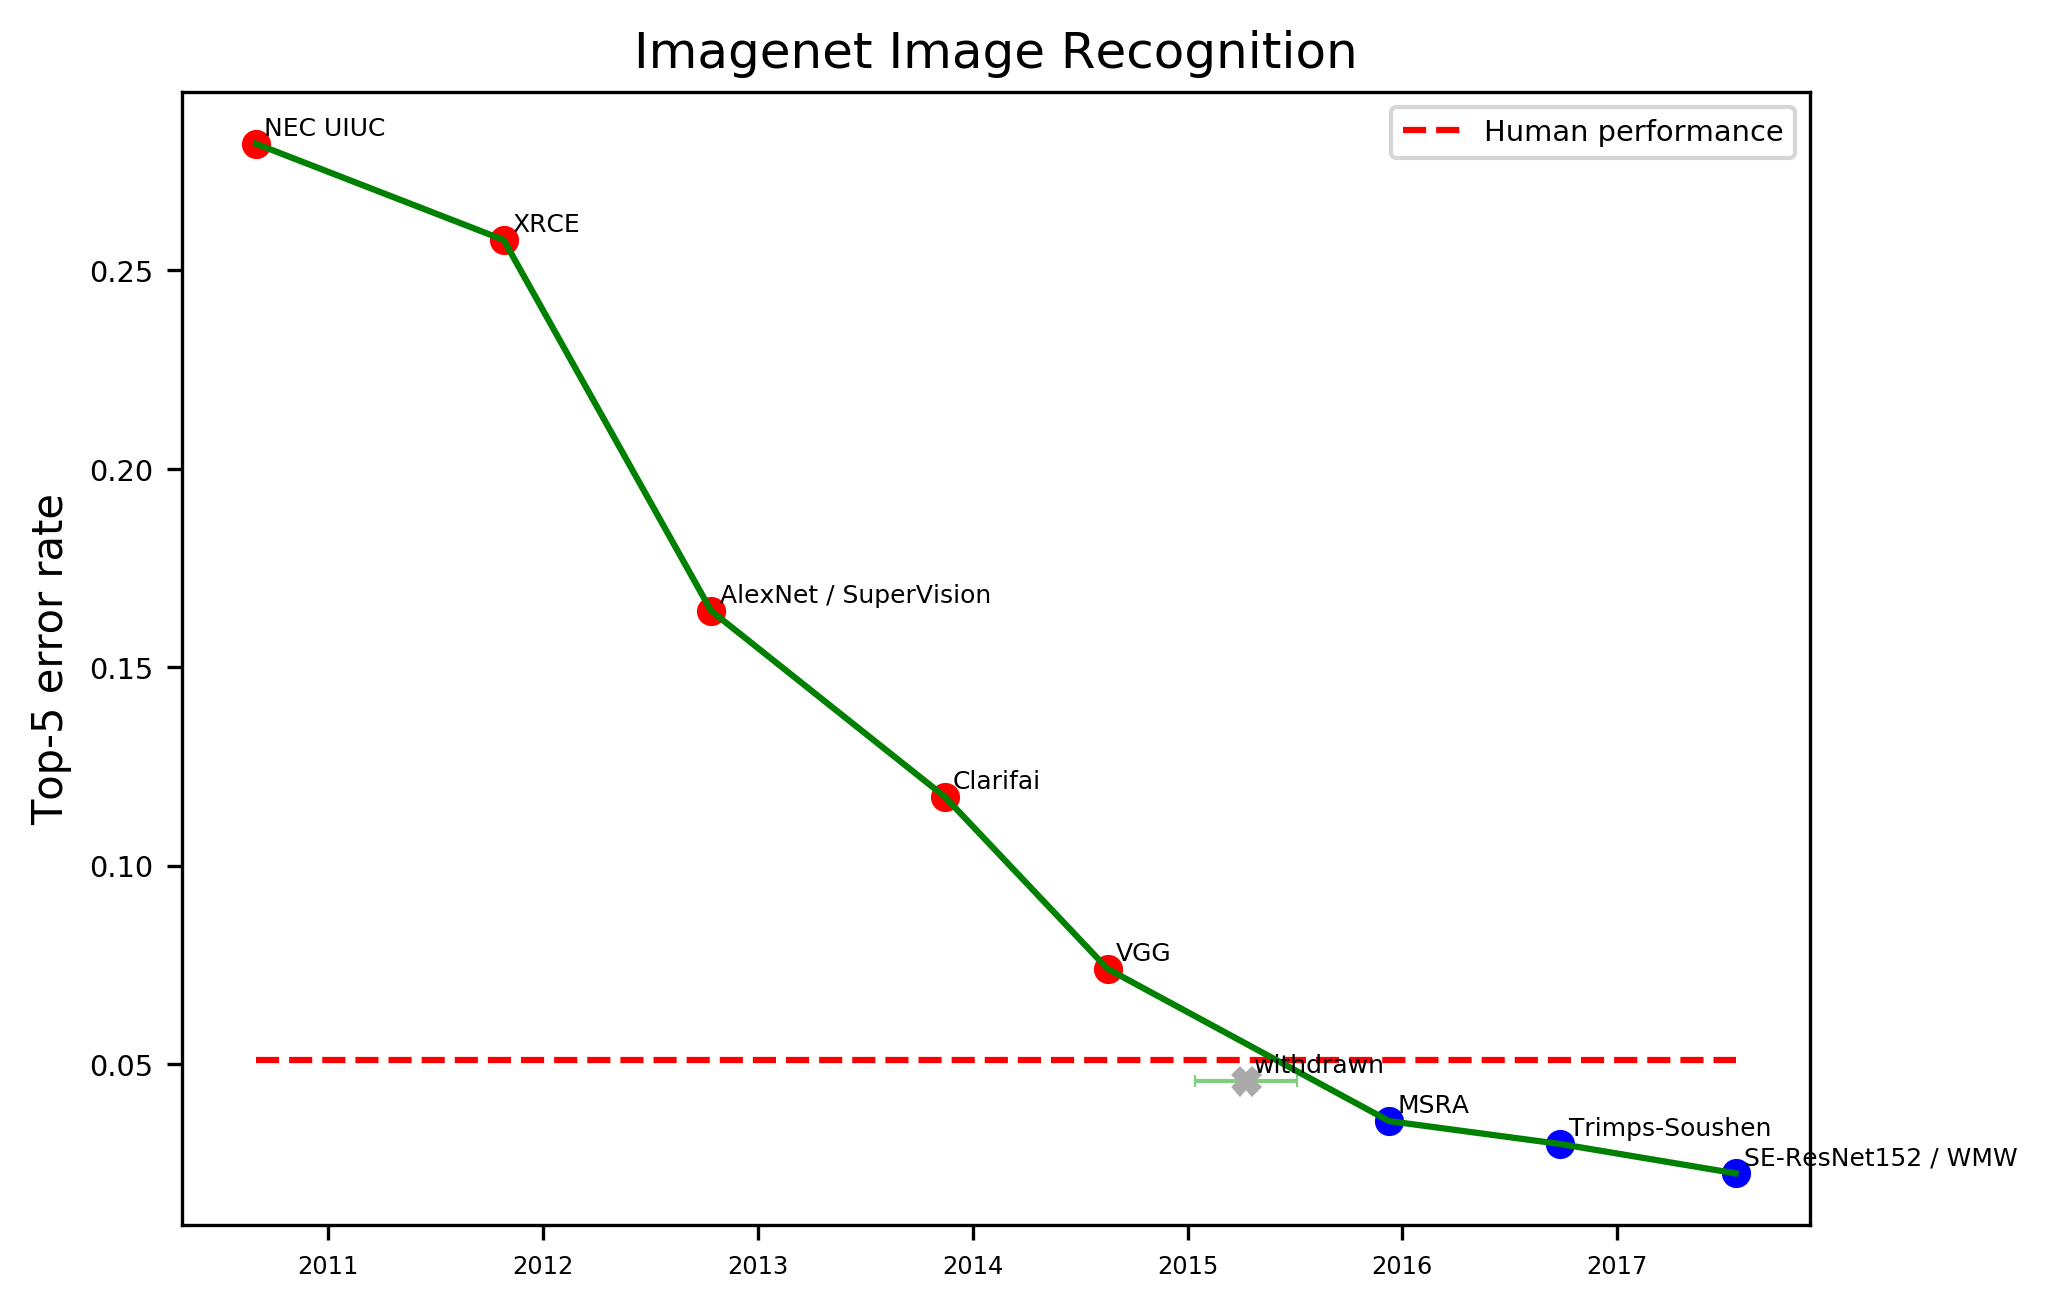
\includegraphics[width=.7\linewidth]{imagenet_recognition.png}
\end{center}
\vfill %
\footnotesize
\color{blue} \url{https://www.eff.org/ai/metrics}
\end{frame} 


\begin{frame}{\# 1. Точность сетей растёт}
\begin{center}
	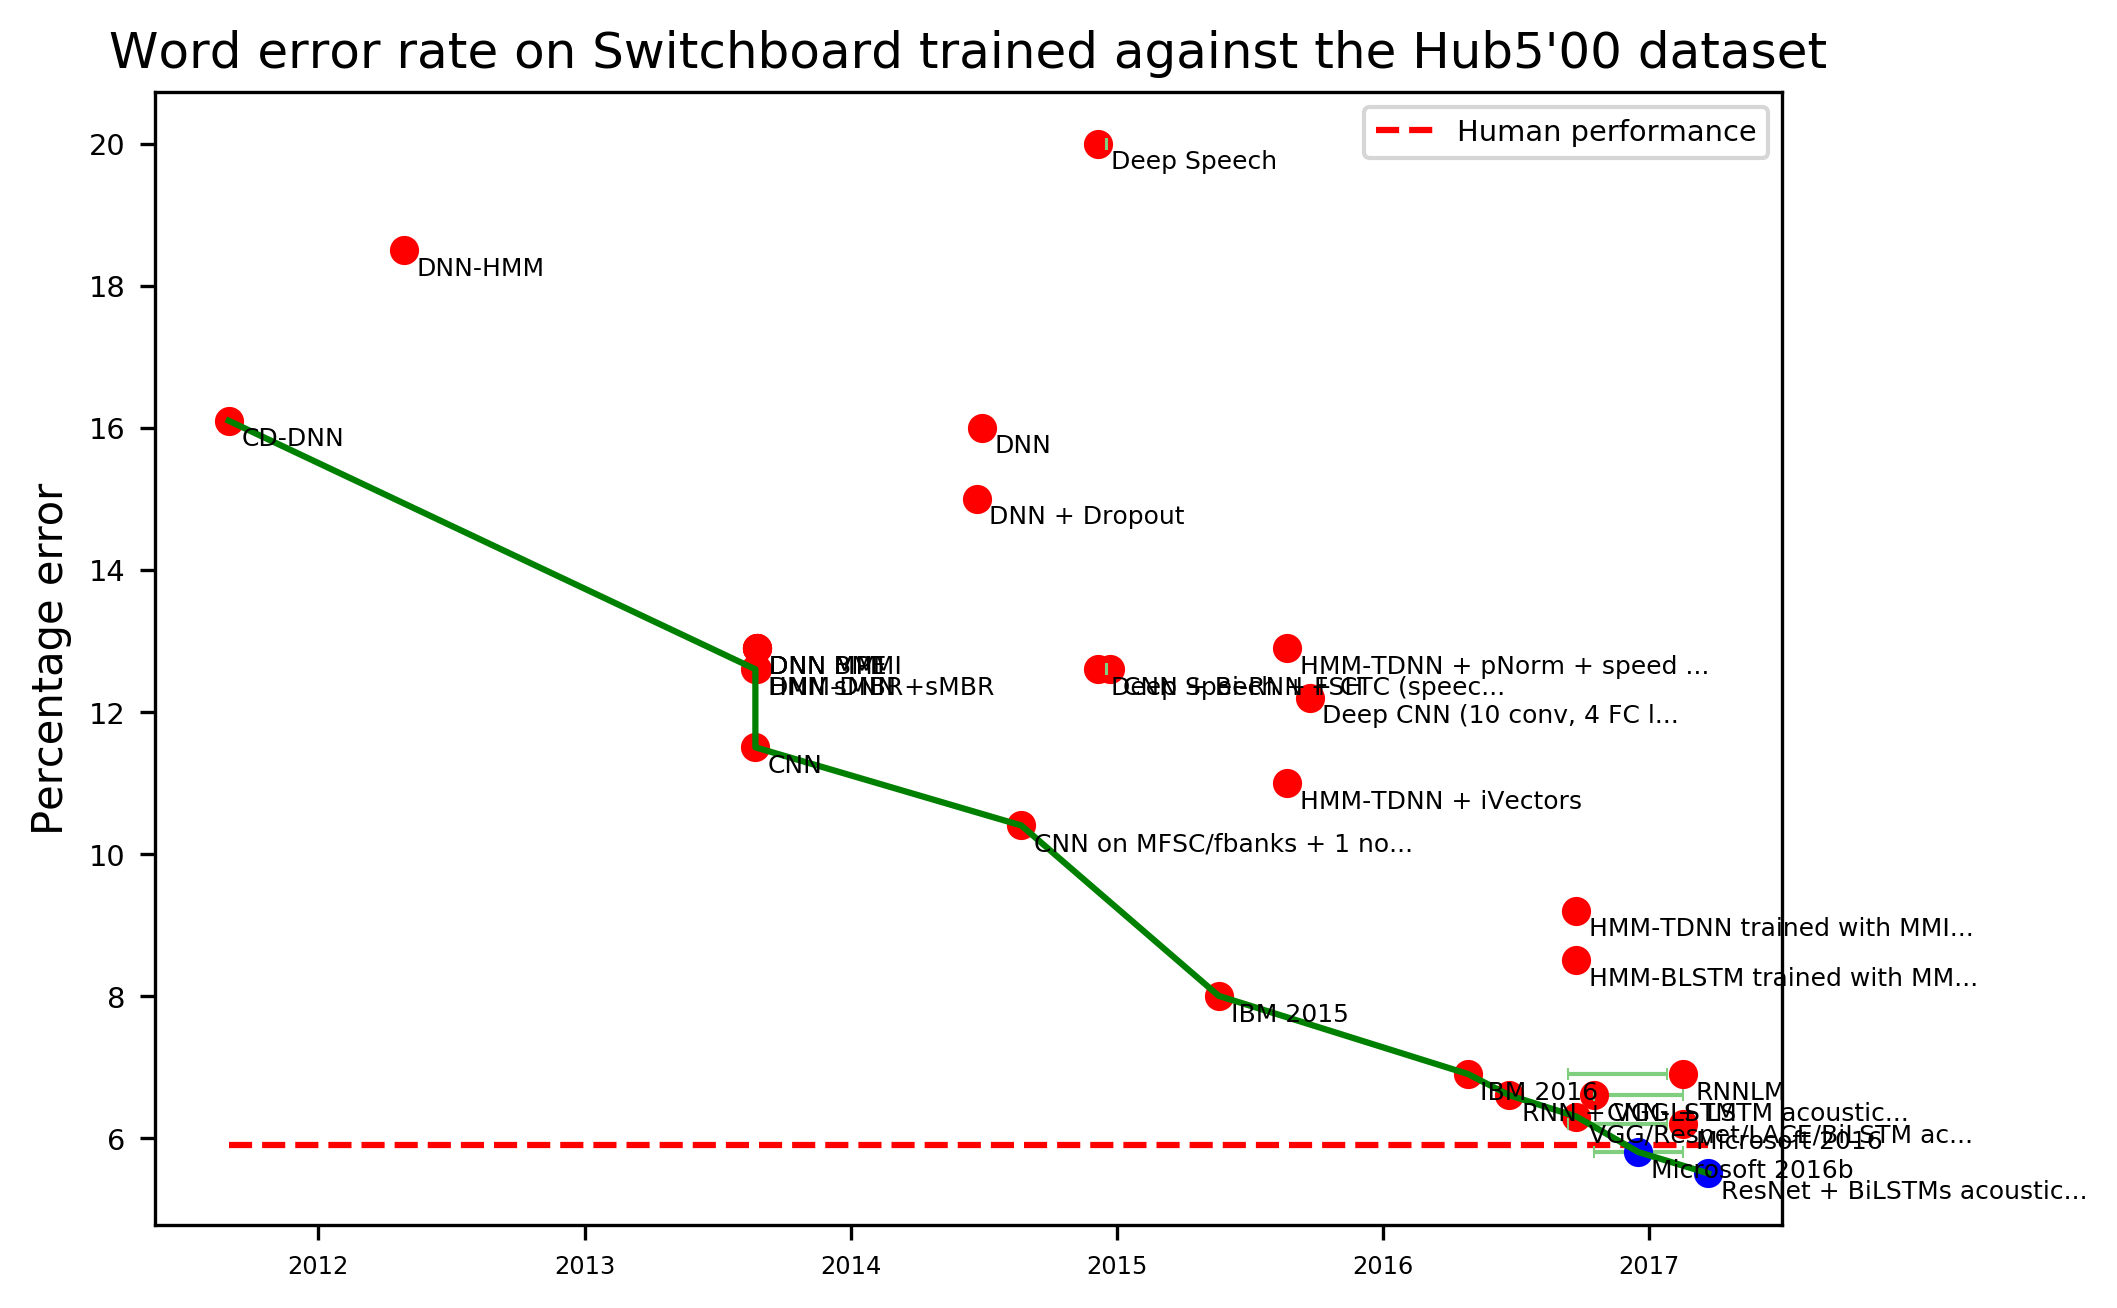
\includegraphics[width=.7\linewidth]{speech_recognition.png}
\end{center}
\vfill %
\footnotesize
\color{blue} \url{https://www.eff.org/ai/metrics}
\end{frame} 


\begin{frame}{\# 2. Сложность сетей растёт}
\begin{center}
	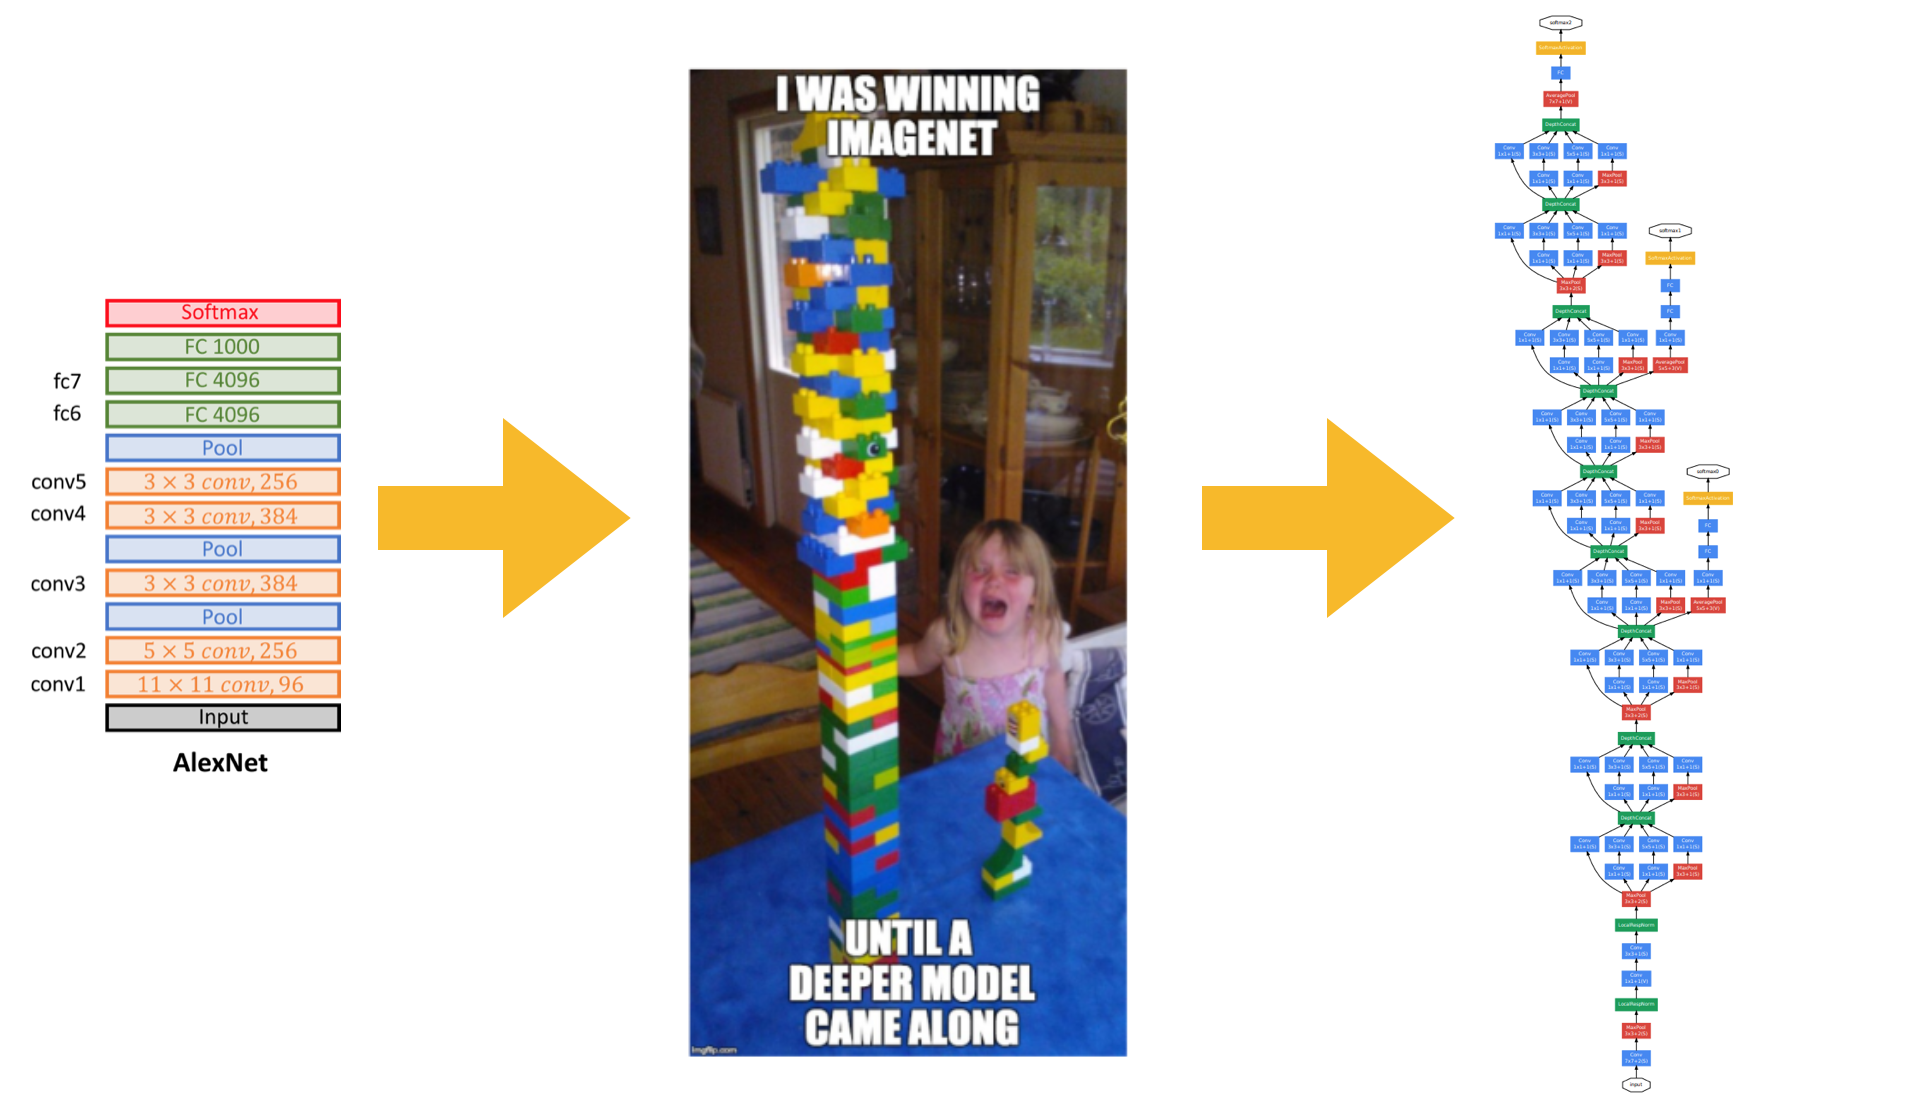
\includegraphics[width=.9\linewidth]{trend2.png}
\end{center}
\end{frame} 


\begin{frame}{\# 2. Сложность сетей растёт}
%\begin{columns}[T] % align columns
%	\begin{column}{.58\textwidth}
\begin{center}
	\includegraphics[width=.67\linewidth]{trend22.png}
\end{center}
%	\end{column}%
%	\hfill%
%\begin{column}{.38\textwidth}
%	\begin{wideitemize}
%		\item размер кружка - число параметров
%		\item по $y$ точность на imagenet
%		\item по $x$ число операций
%	\end{wideitemize}	
%\end{column}%
%\end{columns}
\vfill %
\footnotesize
\color{blue} \url{https://towardsdatascience.com/neural-network-architectures-156e5bad51ba}
\end{frame} 


\begin{frame}{\# 3. Объёмы данных растут}
\begin{center}
	\includegraphics[width=.6\linewidth]{trend3.png}
\end{center}
\vfill %
\footnotesize
\color{blue} \url{https://www.internetlivestats.com}
\end{frame} 


\begin{frame}{\# 4. Вычислительные мощности растут}
\begin{center}
	\includegraphics[width=.6\linewidth]{trend4.png}
\end{center}
\end{frame} 


\begin{frame}{\# 4. Почему это возможно?}
\begin{center}
	\includegraphics[width=.6\linewidth]{trend42.png}
\end{center}
\vfill %
\footnotesize
\color{blue} \url{https://tproger.ru/articles/cpu-and-gpu/}
\end{frame} 


\begin{transitionframe}
	\begin{center}
		\Huge От регрессии к нейросетке 
	\end{center}
	\centering \includegraphics[scale = 0.2]{nn_vas3k.png} 
\end{transitionframe}


\begin{frame}{Линейная регрессия}
\begin{columns}[T] % align columns
	\begin{column}{.38\textwidth}
\begin{center}
	\begin{tikzpicture}[scale = 0.9, line cap=round,line join=round,x=1.0cm,y=1.0cm]
	\draw [line width=1.pt] (0,1.5) circle (0.5cm) node {$1$};
	\draw [line width=1.pt] (2,1.5) circle (0.5cm) node {$x$};
	\draw [line width=1.pt] (1,-1) circle (0.5cm) node {$\hat y$};
	\draw [->, line width=1.pt] (0,1) -- (0.9,-0.4) node[pos=0.3,left] {\small $w_0$};
	\draw [->, line width=1.pt] (2,1) -- (1.1,-0.4) node[pos=0.3,right] {\small $w_1$};
	\end{tikzpicture}

\mbox{ } \\

\begin{equation*}
	\begin{aligned}
& y_i =w_0 + w_1 \cdot x_i \\
& y_i = \begin{pmatrix} 1 & x_i \end{pmatrix} \cdot \begin{pmatrix}  w_0 \\ w_1 \end{pmatrix} \\
& y_i = (x_i, w)\\
	\end{aligned}
\end{equation*}
\end{center}
\end{column}%
\hfill%

\only<1>{\begin{column}{.58\textwidth}
	\begin{center}
		\includegraphics[scale=0.12]{regres.png}
	\end{center}
\end{column}}

\only<2>{\begin{column}{.58\textwidth}
\begin{center}
\begin{equation*}
\begin{aligned}
& y_1 =w_0 + w_1 \cdot x_1 \\
& y_2 =w_0 + w_1 \cdot x_2 \\
& y_3 =w_0 + w_1 \cdot x_3 \\ 
\end{aligned}
\end{equation*}	
\vfill% 
\begin{equation*}
 \begin{pmatrix} y_1 \\ y_2 \\ y_3 \end{pmatrix} =  \begin{pmatrix}  1 & x_1 \\ 1 & x_2 \\ 1 & x_3  \end{pmatrix} \cdot  \begin{pmatrix}  w_0 \\ w_1 \end{pmatrix} 
\end{equation*}		
\vfill% 
%\begin{equation*}
%y = X \cdot w 
%\end{equation*}	
%\vfill% 
\end{center}
\end{column}}
\end{columns}
\end{frame}



\begin{frame}{Линейная регрессия (векторная форма)}
\[
y = \begin{pmatrix} y_1 \\ y_2 \\ \ldots \\ y_n \end{pmatrix}  \qquad X = \begin{pmatrix} 1 & x_{11} & \ldots & x_{1k} \\ 1 & x_{21} & \ldots & x_{2k} \\ \ldots & \ldots & \ldots & \dots \\ 1 & x_{n1} & \ldots & x_{nk} \end{pmatrix}  \qquad  w = \begin{pmatrix} w_0 \\ w_1 \\ \ldots \\ w_k \end{pmatrix} 
\]

Модель: 

\[ 
y = Xw
\]

Оценка: 

\[
\hat w = (X^T X)^{-1} X^T y
\]

Прогноз: 

\[
\hat y = X \hat{w}
\]
\end{frame}


\begin{frame}{Как обучить линейную регрессию?}
\begin{wideitemize}
	
\item Нужно ввести штраф за ошибку: 

\[
MSE(w) = \frac{1}{n} \sum_{i=1}^n (w^T x_i - y_i)^2   \to \min_{w}
\]

\item Не для всех функция потерь бывает аналитическое решение, например для $MAE$ из-за модуля его нет:  

\[ 
MAE(w) = \frac{1}{n} \sum_{i=1}^n |w^Tx_i - y_i|
\]

\item \alert{Обычно модель обучают методом градиентного спуска}
\end{wideitemize} 

\vfill 
\scriptsize Про метрики для регрессии: \\
\color{blue} \url{https://alexanderdyakonov.files.wordpress.com/2018/10/book_08_metrics_12_blog1.pdf}
\end{frame}


\begin{frame}{А что если...}

\begin{columns}[T] % align columns
	\begin{column}{.33\textwidth}

\begin{center}
	\begin{tikzpicture}[line cap=round,line join=round,x=1.0cm,y=1.0cm]
	
	\draw [line width=1.pt] (0,2.5) circle (0.5cm) node {$1$};
	\draw [line width=1.pt] (2,2.5) circle (0.5cm) node {$x$};
	
	\draw [line width=1.pt] (0,-0.5) circle (0.5cm) node {$h_1$};
	\draw [line width=1.pt] (2,-0.5) circle (0.5cm) node {$h_2$};
	
	\draw [line width=1.pt] (1,-3) circle (0.5cm) node {$\hat y$};
	
	\draw [->, line width=1.pt] (0,2) -- (-0.1,0.1) node[pos=0.3,left] {\small $w_{11}$};
	\draw [->, line width=1.pt] (2,2) -- (2.1,0.1) node[pos=0.3,right] {\small $w_{22}$};
	
	\draw [->, line width=1.pt] (0,2) -- (1.9,0.1) node[pos=0.5,left] {\small $w_{12}$};
	\draw [->, line width=1.pt] (2,2) -- (0.1,0.1) node[pos=0.5,right] {\small $w_{21}$};
	
	\draw [->, line width=1.pt] (0,-1) -- (0.8,-2.4) node[pos=0.3,right] {\small $w_{1}$};
	\draw [->, line width=1.pt] (2,-1) -- (1.2,-2.4) node[pos=0.3,left] {\small $w_{2}$};
	\end{tikzpicture}
\end{center}
\end{column}%
\hfill 

\only<1>{\begin{column}{.66\textwidth}
\begin{equation*}
\begin{aligned}
& h_{1i} =w_{11}+ w_{21} \cdot x_i\\
& h_{2i} =w_{12} + w_{22} \cdot x_i \\
& \\
& y_i = w_1 \cdot h_{1i} + w_2 \cdot h_{2i} \\
\end{aligned}
\end{equation*}	
\vfill %
\begin{equation*}
\begin{aligned}
& h = X \cdot W_1 \\
& y = h \cdot W_2 \\
\end{aligned}
\end{equation*}	
\vspace{0.8cm}
\centering 
\Large \alert{Норм идея?}
\end{column}}

\only<2>{\begin{column}{.66\textwidth}
\begin{multline*} 
y = w_1 \cdot h_1 + w_2 \cdot h_2 = \\ = w_1 \cdot (w_{11} + w_{21} \cdot x)  + w_2 \cdot (w_{12} + w_{22} \cdot x)  = \\ = \underbrace{(w_1 w_{11} + w_2 w_{12})}_{\gamma_1} + \underbrace{(w_1 w_{21} + w_2 w_{22})}_{\gamma_2} x 
\end{multline*}
\vspace{0.5cm}
\centering 
{\Large \alert{Чёрт возьми! Опять линейность...} }
\vspace{0.5cm}
\begin{equation*}
y = h \cdot W_2 = X \cdot W_1 \cdot W_2 = X \cdot A
\end{equation*}
\end{column}}

\only<3>{\begin{column}{.66\textwidth}
		\begin{wideitemize}
		\item Давайте добавим к скрытому состоянию какую-нибудь нелинейность: 
	    \end{wideitemize}

		\begin{equation*}
		\begin{aligned}
		& h_{1i} =w_{11}+ w_{21} \cdot x_i\\
		& h_{2i} =w_{12} + w_{22} \cdot x_i \\
		& y_i = w_1 \cdot \alert{f(}h_{1i}\alert{)} + w_2 \cdot \alert{f(}h_{2i}\alert{)} \\
		\end{aligned}
		\end{equation*}	
		\vspace{0.5cm}
		$$
		y = h \cdot W_2 = \alert{f(}X \cdot W_1\alert{)} \cdot W_2 \ne X \cdot A 
		$$
\end{column}}
\end{columns}
\end{frame}



\begin{frame}{Почему нельзя взять такую функцию?}
\begin{center}
	\includegraphics[width=0.7\paperwidth]{activation_1.png}
\end{center}
\end{frame}


\begin{frame}{Сигмоида}
\begin{center}
	\includegraphics[width=0.7\paperwidth]{activation_2.png}
\end{center}
\end{frame}


\begin{frame}{Сигмоида}
\begin{center}
	\includegraphics[width=0.7\paperwidth]{activation_3.png}
\end{center}
\end{frame}


\begin{frame}{Сигмоида}
\begin{wideitemize}
	\item В маленьких сетках сигмоиду можно смело использовать
	\item В глубоких сетях из-за сигмоиды возникает \alert{паралич сети} 
	\item Про него подробнее мы поговорим чуть позже 
	\item Нужна другая нелинейная функция активации 
\end{wideitemize}
\end{frame}


\begin{frame}{От линейной активации ... }
\begin{center}
	\includegraphics[width=0.7\paperwidth]{activation_1.png}
\end{center}
\end{frame}


\begin{frame}{... к нелинейной}
\begin{center}
	\includegraphics[width=0.7\paperwidth]{activation_4.png}
\end{center}
\end{frame}


{
	\usebackgroundtemplate{ 
		\includegraphics[width=\paperwidth]{activation_5.png}}
	\begin{frame}{ReLU}  \pause 
	\vspace{7.4cm}
	\hspace{3cm} \footnotesize \alert{Эта шутка была мною нагло украдена у моего друга Ильи Езепова}
	\end{frame}
}


\begin{transitionframe}
	\begin{center}
		\Huge Персептрон \\ \mbox{ } \\
		\includegraphics[scale=0.25]{artifitial_idiot.jpg}
	\end{center}
\end{transitionframe}


\begin{frame}{Нейрон}
\begin{center}
		\includegraphics[width=0.55\paperwidth]{brain_neuron.png} \\
		\Large \alert{Хватит нам врать!}
\end{center}
\end{frame}


\begin{frame}{Мышь Розенблата}
\begin{columns}[T] 
\begin{column}{.49\textwidth}
	\begin{wideitemize}
		\item Термин нейронная сеть пришёл из биологии, его придумали $70$ лет назад
		\item  Оказалось, что мозг устроен гораздо сложнее
		\item  Продуктивнее думать про нейросетки,  как про вычислительные графы
	\end{wideitemize}
\end{column}
\begin{column}{.49\textwidth}
	\begin{center}
		\includegraphics[scale=0.35]{rozen_mouse.png}  \\ 
		\Large \alert{Не забыли его?} 
	\end{center}
\end{column}
\end{columns}
\vfill %
\footnotesize 
\color{blue} \url{https://habr.com/ru/company/mailru/blog/405615/}
\end{frame}


\begin{frame}{Перcептрон Розенблатта (1950)}
	\begin{center}
		\includegraphics[width=0.55\paperwidth]{neuron_1.png}
	\end{center}
	\[
	y = \begin{cases}
	1, \text{ если } \sum w_i x_i \ge \gamma \\
	0, \text{ если } \sum w_i x_i < \gamma \\
	\end{cases}
	\]
\end{frame}


\begin{frame}{Функция активации}
	\begin{center}
	 \includegraphics[width=0.51\linewidth]{neuron_3.png}
	\end{center}
	\begin{itemize}
		\item Функция активации $\sigma(t)$ вносит нелинейность, она может быть любой
	\end{itemize}
\end{frame}


\begin{frame}{Линейная регрессия}
\begin{columns}[T] 
	\begin{column}{.45\textwidth}
		\begin{center}
			\includegraphics[width=0.99\linewidth]{neuron_3.png}
		\end{center}
	\end{column}%
	\hfill%
	\begin{column}{.55\textwidth}
		Нейрон с линейной функции активации~—   это линейная регрессия... 
		\begin{equation*}
		\begin{aligned}
		& \sigma(t) = t \\
		& y= w_0 + w_1 \cdot x_1 + \ldots + w_n \cdot x_n \\
		\end{aligned}
		\end{equation*}
	\end{column}%
\end{columns}
\end{frame}


\begin{frame}{Логистическая регрессия}
\begin{columns}[T] 
	\begin{column}{.45\textwidth}
		\begin{center}
			\includegraphics[width=0.99\linewidth]{neuron_3.png}
		\end{center}
	\end{column}%
	\hfill%
	\begin{column}{.55\textwidth}
%		\alert{Про классификацию подробнее в следущий раз} \\ 
%		
%		\mbox{ } \\ 
		
		Нейрон с сигмоидом в качестве функции активации — это логистическая регрессия... 
		\begin{equation*}
		\begin{aligned}
		& \sigma(t) = \frac{1}{1 + e^{-t}} \\
		& P(y = 1 \mid x) = \sigma(w_0 + w_1 \cdot x_1 + \ldots + w_n \cdot  x_n) \\
		\end{aligned}
		\end{equation*}
	\end{column}%
\end{columns}
\end{frame}


\begin{frame}{Функция активации}
	\begin{center}
		\includegraphics[width=0.51\linewidth]{neuron_3.png}
	\end{center}
	\begin{equation*}
		\begin{aligned}
		y &= \sigma(X \cdot W) \\ 
		\end{aligned}
	\end{equation*}
\end{frame}


\begin{frame}{Две регрессии скрепили третьей}
	\begin{center}
		\includegraphics[width=0.7\paperwidth]{neuron_4.png}
	\end{center}
	\begin{equation*}
		\begin{aligned}
		& h_j = \sigma(w_0 + w_{j1}^1 \cdot x_1 + \ldots + w_{jk}^1 \cdot x_k)\\
		& y = \sigma(w_{11}^2 \cdot h_1 + w_{21}^2 \cdot h_2) \\
		\end{aligned}
	\end{equation*}
\end{frame}


\begin{frame}{MLP (multi-layer perceptron)}
	\begin{center}
		\includegraphics[width=0.7\paperwidth]{neuron_4.png}
	\end{center}
	\begin{equation*}
		\begin{aligned}
		&h = \sigma(X \cdot W) \\
		&y = \sigma(h \cdot W) \\
		\end{aligned}
	\end{equation*}
\end{frame}


\begin{frame}{Армия из регрессий}
	\begin{center}
		\includegraphics[width=0.8\paperwidth]{network.png}
	\end{center}
\end{frame}


\begin{frame}{The Perceptron Convergence Theorem (Rosenblat, 1965)}
	\begin{wideitemize}
		\item Любая непрерывная и ограниченная функция может быть сколь угодно точно аппроксимирована нейронной сетью с одним скрытым слоем с нелинейной функцией активации нейрона.
		
		\item Любая функция может быть сколь угодно точно аппроксимирована нейронной сетью с двумя скрытыми слоями с нелинейной функцией активации нейрона.
		
		\item Что ещё можно пожелать?
	\end{wideitemize}

\vfill %
\footnotesize Графическое доказательство теоремы:  \\
\color{blue} \url{http://neuralnetworksanddeeplearning.com/chap4.html}
\end{frame}


{
	\usebackgroundtemplate{ 
		\includegraphics[width=\paperwidth]{goingdeeper.jpg}}
	\begin{frame}[fragile]
	\vspace{6.5cm}
	\begin{center}
		{\color{white} \Huge{Going Deeper}}
	\end{center}
\end{frame}
}


\begin{frame}{Мотивация}
	\begin{wideitemize}
		\item Персептрон может решить любую проблему, но это дорого
		
		\item Глубокие архитектуры часто позволяют выразить то же самое, приблизить те же функции гораздо более эффективно, чем неглубокие
		
		\item Каждый новый слой сетки будет работать всё с более сложными фичами
	\end{wideitemize}
\end{frame}


\begin{frame}{Армия из регрессий}
	\begin{center}
		\includegraphics[width=0.73\paperwidth]{network_1.png}
	\end{center}
\end{frame}


\begin{frame}{MLP не отходя от браузера}
\begin{center}
	\includegraphics[width=0.76\paperwidth]{tensorflow_demo.png}
\end{center}
\vfill %
\footnotesize 
\color{blue} \url{http://playground.tensorflow.org}
\end{frame}


\begin{frame}{MLP не отходя от браузера}
\begin{center}
	\includegraphics[width=0.76\paperwidth]{tensorflow_demo2.png}
\end{center}
\vfill %
\footnotesize 
\color{blue} \url{http://playground.tensorflow.org}
\end{frame}


\begin{frame}{Ещё одна аналогия}
\begin{center}
\begin{tikzpicture}
\node[inner sep=0pt] (russell) at (0,0)
{\includegraphics[width=0.95\paperwidth]{bumaga.png}};
%\node[] at (4,3) {{\fontsize{2}{60}\selectfont Ты пидор} };
\end{tikzpicture}
\end{center}
\end{frame}


\begin{transitionframe}
	\begin{center}
		\Huge Нейросети  — конструктор LEGO
	\end{center}
	\centering \includegraphics[scale = 0.4]{lego_title.png}
\end{transitionframe}


\begin{frame}{Слои бывают разными}
	\begin{wideitemize}
		\item Слой, который просто взвешивает входы называется \alert{полносвязным.}
		
		\item Слои бывают очень разными. Например, \alert{Dropout:}  с вероятностью $p$ отключаем нейрон. Такой слой препятствует переобучению и делает нейроны более устойчивыми к случайным возмущениям.
	\end{wideitemize}
	\begin{center}
		\includegraphics[width=0.3\paperwidth]{dropout.png}
	\end{center}
\end{frame}


\begin{frame}{Функции активации бывают разными}
\begin{center}
	\includegraphics[width=0.7\paperwidth]{activations.png}
\end{center}
\end{frame}


\begin{frame}{Архитектуры бывают разными}
	\begin{center}
		\includegraphics[width=0.75\paperwidth]{nn_lego_1.png}
	\end{center}
	Каждый слой — просто функция, каждая сетка — конструктор LEGO
\end{frame}


\begin{frame}{Регрессия}
\begin{center}
	\includegraphics[width=0.75\paperwidth]{nn_lego_1.png}
\end{center}
\end{frame}

\begin{frame}{Мультирегрессия}
\begin{center}
	\includegraphics[width=0.75\paperwidth]{nn_lego_regr.png}
\end{center}
\end{frame}



\begin{frame}{Классификация}
	\begin{center}
		\includegraphics[width=0.75\paperwidth]{lego_class_two.png}
	\end{center}
\end{frame}


\begin{frame}{Классификация}
\begin{wideitemize}
	\item  $y \in \{0, 1 \}$ — целевая переменная,  $X$ — признаки  
	
	\only<1-2>{
		\item Модель:   $y = w_0 + w_1 x_1 + w_2 x_2 + \ldots + w_k x_k $
	}
	
	\only<3>{
		\item Модель:   $y =  \left[ w_0 + w_1 x_1 + w_2 x_2 + \ldots + w_k x_k  > \gamma \right] $
	}
	
	\only<4>{
		\item Модель:   $\alert{P(y = 1 \mid w)} = F \left( w_0 + w_1 x_1 + w_2 x_2 + \ldots + w_k x_k  \right)$
	}
\end{wideitemize} 

\only<2>{
	\begin{center}
		\includegraphics[width= 0.5\linewidth]{logreg_problem.png}
	\end{center}
}

%\only<3>{
%	\begin{center}
%		\includegraphics[width= 0.5\linewidth]{logreg_hinge.png}
%	\end{center}
%}

\only<3>{
	\begin{center}
		\includegraphics[width= 0.5\linewidth]{logreg_solveprob.png}
	\end{center}
}

\only<4>{
	\begin{columns}[T] %
		\begin{column}{.5\textwidth}
			\begin{center}
				\includegraphics[width= 0.95\linewidth]{logreg_solveprob.png}
			\end{center}
		\end{column}%
		\hfill%
		\begin{column}{.5\textwidth}
			
			\begin{itemize}
				\item В качестве $F(t)$ можно взять любую функцию распределения
				\item Если взять сигмоиду, модель будет интерпретируемая
			\end{itemize}
			
			\begin{equation*}
			\begin{aligned}
			& F(t) =  \sigma(t) =  \frac{1}{1 + e^{-t}} =  \frac{e^t}{1 + e^{t}} \\
			& \sigma'(t) = \sigma(t) \cdot  (1 - \sigma(t)) 
			\end{aligned}
			\end{equation*} 
		\end{column}%
	\end{columns}
}
\end{frame}


\begin{frame}{Сигмоида}
\begin{center}
	\begin{tikzpicture}
	\begin{axis}[
	legend pos=north west,
	axis x line=middle,
	axis y line=middle,
	yticklabels=\empty,
	xticklabels=\empty,
	%		x tick label style={/pgf/number format/fixed,
	%			/pgf/number format/fixed zerofill,
	%			/pgf/number format/precision=1},
	%		y tick label style={/pgf/number format/fixed,
	%			/pgf/number format/fixed zerofill,
	%			/pgf/number format/precision=1},
	grid = major,
	width=14cm,
	height=7cm,
	grid style={dashed, gray!30},
	xmin=-1,     % start the diagram at this x-coordinate
	xmax= 1,    % end   the diagram at this x-coordinate
	ymin= 0,     % start the diagram at this y-coordinate
	ymax= 1,   % end   the diagram at this y-coordinate
	%axis background/.style={fill=white},
	%		xlabel=x,
	%		ylabel=y,
	%tick align=outside,
	enlargelimits=false]
	
	% plot the stirling-formulae
	\addplot[domain=-1:1, red, ultra thick,samples=500] {1/(1+exp(-5*x))};
	\addplot[domain=-1:1, blue, ultra thick,samples=500] {1/(1+exp(-10*x))};
	\addlegendentry{$f(t)=\frac{1}{1+e^{-5t}}$}
	\addlegendentry{$g(t)=\frac{1}{1+e^{-10t}}$}
	\end{axis}
	\end{tikzpicture}
\end{center}
\end{frame}


%  Хардовый вариант
%\begin{frame}{Функция потерь}
%\begin{equation*} 
%\begin{aligned}
%L(w) &=P(y_1, \ldots, y_n \mid X, w) =  \\ 
%&= P(y_1 \mid X,w) \cdot \ldots \cdot P(y_n \mid X, w) =  \\ 
%&= p^{\sum y_i} \cdot (1-p)^{n - \sum y_i} \to \max_{w} \\ 
%\mbox{ } \\  \pause 
%\ln L(w) & = \sum y_i \cdot \ln p + \sum(1 - y_i) \cdot \ln(1-p) = \\ 
%&= \sum [ y_i \cdot \ln p + (1 - y_i) \cdot \ln(1-p)] \to \max_{w} \\
%\mbox{ } \\  \pause 
%\logloss(w) & = -\ln L(w) = - \sum [ y_i \cdot \ln p + (1 - y_i) \cdot \ln(1-p)]  \to \min_{w}  \\  \pause 
%p &= P(y_i = 1 \mid X, w) =  \sigma(x_i^T w) = \frac{1}{1 + e^{-x_i^T w}}  \\ 
%\mbox{ } \\ 
%\end{aligned}
%\end{equation*}
%\end{frame}


% Простой вариант 
\begin{frame}{Функция потерь}
	\begin{columns}[T] %
	\begin{column}{.5\textwidth}
		\begin{wideitemize}
			\item Наши $y$ принимают значения $0$ и $1$ 
			\item Если $y = 1$, хотим большое $\hat p = \hat P(y = 1)$, но чем ближе $\hat p$ к $1$, тем меньше хотим его увеличить 
			\item Если $y = 0$, хотим большое $(1 - \hat p)$, получается функция потерь: 
			
			$$
			\logloss = - \frac{1}{n} \sum_{i=1}^n y_i \cdot \ln \hat p + (1 - y_i) \cdot \ln (1 - \hat p)
			$$
		\end{wideitemize}	
	\end{column}%
	\hfill%
	\begin{column}{.5\textwidth}
		\begin{center}
			\includegraphics[width= 0.95\linewidth]{log_loss_05.png}
		\end{center}
	\end{column}%
\end{columns}
\end{frame}



\begin{frame}{Пример: два класса}
\begin{tabular}{m{2.5cm} m{0.35cm} m{1.8cm} m{0.35cm} m{0.5cm} m{0.35cm} m{0.8cm}  m{0.5cm} m{3.2cm}} 
	
	& & & &  {\large  $\mbox{ }t$ } &  &  {\large $\sigma(t)$} &  &  {\large \only<1>{\hspace{20pt}} logloss} \\
	\includegraphics[scale=0.2]{tab_cat.png} & {\Large $\Rightarrow$} & \includegraphics[scale=0.2]{tab_nn.png}  &  {\Large $\Rightarrow$} &  $10$ &  {\Large $\Rightarrow$} &  \only<1>{$0.99$}  & {\Large $\Rightarrow$}  & \only<1>{ \begin{equation*} \begin{aligned} &- (1 \cdot \ln 0.99 + \\ &(1 - 1) \cdot \ln (1 - 0.99)) \end{aligned} \end{equation*}} \\
	
	\includegraphics[scale=0.2]{tab_dog.png}&  {\Large $\Rightarrow$} &  \includegraphics[scale=0.2]{tab_nn.png}  &  {\Large $\Rightarrow$}  &  $-1$ &  {\Large $\Rightarrow$}  &  \only<1>{$0.26$}  & {\Large $\Rightarrow$}  &  \only<1>{ \begin{equation*} \begin{aligned} &-(0 \cdot \ln 0.26 + \\ & (1 - 0) \cdot \ln(1 - 0.26))\end{aligned} \end{equation*}}  \\
\end{tabular}
\end{frame}


%% ГОВНОКОООД и КОПИПАСТААА
\begin{frame}{Пример: два класса}
\begin{tabular}{m{2.5cm} m{0.35cm} m{1.8cm} m{0.35cm} m{0.5cm} m{0.35cm} m{2cm}  m{0.5cm} m{3.2cm}} 
	& & & &  {\large  $\mbox{ }t$ } &  &  {\large \hspace{8pt} $\sigma(t)$} &  &  {\large logloss} \\
	\includegraphics[scale=0.2]{tab_cat.png} & {\Large $\Rightarrow$} & \includegraphics[scale=0.2]{tab_nn.png}  &  {\Large $\Rightarrow$} &  $10$ &  {\Large $\Rightarrow$} &  $[\alert{0.99}, 0.01]$ & {\Large $\Rightarrow$}  & $-\ln 0.99$ \\
	
	\includegraphics[scale=0.2]{tab_dog.png}&  {\Large $\Rightarrow$} &  \includegraphics[scale=0.2]{tab_nn.png}  &  {\Large $\Rightarrow$}  &  $-1$ &  {\Large $\Rightarrow$}  &   $[0.26, \alert{0.74}]$ & {\Large $\Rightarrow$}  &  $-\ln 0.74$\\
\end{tabular}
\end{frame}


\begin{frame}{Мультиклассификация}
\begin{center}
	\includegraphics[width=0.75\paperwidth]{lego_nn_multi.png}
\end{center}
\end{frame}


\begin{frame}{Мультиклассификация}
\begin{center}
\includegraphics[width=0.9\paperwidth]{softmax.png}
\end{center}
\end{frame}


\begin{frame}{Softmax (мягкий максимум)}

Много классов, $y \in {1, \ldots, K}$

\begin{equation*}
\begin{aligned}
(w_1^T x, &\ldots, w_K^Tx) \\
&\Downarrow \\
(e^{z_1}, &\ldots, e^{z_K}) \\
&\Downarrow \\
\left(\frac{e^{z_1}}{\sum_{k=1}^K e^{z_k}}\right., &\ldots,\left. \frac{e^{z_K}}{\sum_{k=1}^K e^{z_k}}  \right)
\end{aligned}
\end{equation*}

Потери (кросс-энтропия): 

\[
\logloss =  - \sum_{i=1}^n \sum_{k=1}^K [y_i = k] \cdot \ln \frac{e^{w_k^Tx_i}}{\sum_{j=1}^{K} e^{w_j^Tx_i}}
\]
\end{frame}


\begin{frame}{Пример: три класса}
\begin{tabular}{m{2.5cm} m{0.35cm} m{1.8cm} m{0.35cm} m{1cm} m{0.35cm} m{2.7cm} m{0.5cm} m{1.5cm}} 

& & & &  {\large  $\mbox{ }t$ } &  &  {\large \hspace{5pt} Softmax} &  &  {\large  logloss} \\
\includegraphics[scale=0.2]{tab_cat.png} & {\Large $\Rightarrow$} & \includegraphics[scale=0.2]{tab_nn.png}  &  {\Large $\Rightarrow$} &  $[5, 4, 2]$ &  {\Large $\Rightarrow$} &  $[\alert{0.71}, 0.26, 0.04]$ & {\Large $\Rightarrow$}  & $-\ln 0.71$\\

\includegraphics[scale=0.2]{tab_dog.png}&  {\Large $\Rightarrow$} &  \includegraphics[scale=0.2]{tab_nn.png}  &  {\Large $\Rightarrow$}  &  $[4, 2, 8]$ &  {\Large $\Rightarrow$}  & $[0.02, 0.00, \alert{0.98}]$ & {\Large $\Rightarrow$}  & $-\ln 0.98$\\

\includegraphics[scale=0.2]{tab_fox.png} & {\Large $\Rightarrow$} & \includegraphics[scale=0.2]{tab_nn.png}  &  {\Large $\Rightarrow$} &  $[4, 4, 1]$ &  {\Large $\Rightarrow$} &  $[0.49, \alert{0.49}, 0.02]$ & {\Large $\Rightarrow$}  & $-\ln 0.49$\\
\end{tabular}
\end{frame}


\begin{frame}{Важный нюанс}
\begin{wideitemize} 
\item При поиске Softmax мы ищем экспоненты, в памяти компьютера может произойти переполнение из-за больших чисел

\item  Если добавить ко всем входам нейронки одинаковую константу, значение Sofrmax не изменится: 

\[ 
\frac{e^{z_i + c}}{\sum_{k=1}^K e^{z_k + c}} = \frac{ e^c \cdot e^{z_i } }{e^c \cdot \sum_{k=1}^K e^{z_k} }   = 	\frac{e^{z_i}}{\sum_{k=1}^K e^{z_k }} 
\] 

\item  Обычно считают устойчивый к переполнению Softmax: 

\[
\Softmax(z_1, \ldots, z_{K}) = \Softmax(z_1 - \max_i (z_i), \ldots, z_{K} - \max_i (z_i))
\]

\end{wideitemize}
\end{frame}


\begin{frame}{Нейросети -  конструктор LEGO}
\begin{center}
	\includegraphics[width=0.8\paperwidth]{lego_lego.png}
\end{center}
\end{frame}


\begin{transitionframe}
	\begin{center}
		\Huge Учим свою первую нейросеть!
	\end{center}
\end{transitionframe}

\end{document}


